\documentclass[11pt, a4paper]{report}
\usepackage{preamble}

\title{%
    \textbf{ISIS-1611: Inteligencia Artificial}\\[0.5em]
    \large Notas del Curso --- Semestre 2026-19\\
    \normalsize Universidad de los Andes\\
    \normalsize Basado en: \textit{Artificial Intelligence: A Modern Approach}\\
    \normalsize Russell, Norvig \& Ming-Wei Chang (4ª ed.)
}
\author{Carla González}
\date{\today}

\begin{document}

\maketitle
\tableofcontents
\newpage

% =============================================
% PARTE 1: Búsqueda
% =============================================
\part{Búsqueda}

% =============================================
% SEMANA 1
% Temas: Contexto e Historia IA, Agentes Inteligentes,
%        Búsqueda Desinformada (Cap. 1-2, 3.1-3.5)
% =============================================
\chapter{Semana 1: Introducción y Búsqueda Desinformada}

% Clase 1 — Contexto, Historia IA y Agentes Inteligentes
% Lectura: AIMA Cap. 1-2
\section{Contexto e Historia de la IA}

\subsection{Impacto de la IA en el mundo real}

La IA impacta múltiples sectores: economía, política, ley y derecho, trabajo, ciencia, salud y educación.

\subsection{¿Qué es la Inteligencia Artificial?}

Existen cuatro enfoques para definir la IA:

\begin{center}
\begin{tabular}{|l|l|}
\hline
\textbf{Pensamiento humano} & \textbf{Pensamiento racional} \\
Modelos cognitivos & Leyes del pensamiento (lógica) \\
\hline
\textbf{Actuar humanamente} & \textbf{Actuar racionalmente} \\
Test de Turing & Agentes racionales \\
\hline
\end{tabular}
\end{center}

\begin{remark}
La IA moderna se enfoca en \textbf{agentes racionales}: entidades que perciben su entorno y actúan para maximizar su medida de desempeño esperada.
\end{remark}

\subsection{Historia de la IA}

\begin{figure}[H]
\centering
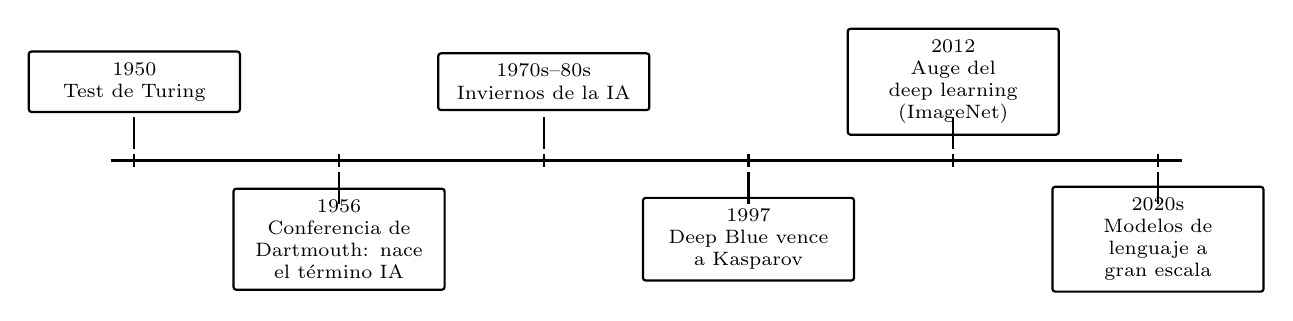
\begin{tikzpicture}[
  hito/.style={draw=black, thick, rectangle, rounded corners=1pt, inner sep=4pt, font=\scriptsize, text width=2.4cm, align=center}
]
\draw[thick] (-0.3,0) -- (13.3,0);
\foreach \x in {0,2.6,5.2,7.8,10.4,13} \draw[thick] (\x,0.08) -- (\x,-0.08);

\node[hito] at (0,1.0)    {1950\\Test de Turing};
\node[hito] at (2.6,-1.0) {1956\\Conferencia de Dartmouth: nace el término IA};
\node[hito] at (5.2,1.0)  {1970s--80s\\Inviernos de la IA};
\node[hito] at (7.8,-1.0) {1997\\Deep Blue vence a Kasparov};
\node[hito] at (10.4,1.0) {2012\\Auge del deep learning (ImageNet)};
\node[hito] at (13,-1.0)  {2020s\\Modelos de lenguaje a gran escala};

\draw[thick] (0,0.15)   -- (0,0.55);
\draw[thick] (2.6,-0.15) -- (2.6,-0.55);
\draw[thick] (5.2,0.15) -- (5.2,0.55);
\draw[thick] (7.8,-0.15) -- (7.8,-0.55);
\draw[thick] (10.4,0.15) -- (10.4,0.55);
\draw[thick] (13,-0.15) -- (13,-0.55);
\end{tikzpicture}
\caption{Línea de tiempo con algunos hitos de la historia de la IA.}
\end{figure}

\section{Agentes Inteligentes}
% Lectura: AIMA Cap. 2

\subsection{¿Qué es un Agente?}

\begin{definition}[Agente]
Un agente es cualquier entidad que \textbf{percibe} su ambiente mediante \textbf{sensores} y \textbf{actúa} sobre él mediante \textbf{actuadores}.
\end{definition}

La función del agente mapea percepciones a acciones: $f: P^* \rightarrow A$

\begin{figure}[H]
\centering
\begin{tikzpicture}[
  caja/.style={draw=black, thick, rectangle, rounded corners=1pt, minimum width=3cm, minimum height=1.4cm, font=\small}
]
\node[caja] (agente) at (0,0) {Agente};
\node[caja] (ambiente) at (6,0) {Ambiente};

\draw[-{Latex},thick] ([yshift=4mm]ambiente.west) -- node[above, font=\scriptsize]{Sensores (percepción)} ([yshift=4mm]agente.east);
\draw[-{Latex},thick] ([yshift=-4mm]agente.east) -- node[below, font=\scriptsize]{Actuadores (acción)} ([yshift=-4mm]ambiente.west);
\end{tikzpicture}
\caption{Ciclo agente-ambiente: el agente percibe el ambiente a través de sensores y actúa sobre él mediante
actuadores, en un ciclo continuo.}
\end{figure}

\begin{example}[PEAS de un taxi autónomo]
    La descripción PEAS de un taxi autónomo es:
    \begin{itemize}
        \item \textbf{Performance}: seguridad, tiempo de viaje, cumplir normas de tránsito, comodidad del pasajero.
        \item \textbf{Environment}: calles, otros vehículos, peatones, señales de tránsito, clima.
        \item \textbf{Actuators}: dirección, acelerador, freno, señales, bocina.
        \item \textbf{Sensors}: cámaras, GPS, velocímetro, sensores de proximidad (LIDAR/radar).
    \end{itemize}
\end{example}

\subsection{Racionalidad}

Un agente racional selecciona la acción que maximiza su \textbf{medida de desempeño} esperada, dado su conocimiento actual.

Depende de:
\begin{enumerate}
    \item La medida de desempeño
    \item El conocimiento previo del entorno
    \item Las acciones disponibles
    \item La secuencia de percepciones hasta el momento
\end{enumerate}

\subsection{Descripción PEAS}

Para caracterizar el ambiente de una tarea se usa PEAS:
\begin{itemize}
    \item \textbf{P}erformance (Medida de desempeño)
    \item \textbf{E}nvironment (Entorno)
    \item \textbf{A}ctuators (Actuadores)
    \item \textbf{S}ensors (Sensores)
\end{itemize}

\subsection{Naturaleza de los Ambientes}

\begin{tabular}{ll}
\toprule
\textbf{Dimensión} & \textbf{Valores posibles} \\
\midrule
Observabilidad & Completamente observable / Parcialmente observable \\
Agentes & Un solo agente / Multiagente \\
Determinismo & Determinista / Estocástico \\
Episodicidad & Episódico / Secuencial \\
Dinamismo & Estático / Dinámico \\
Tiempo & Discreto / Continuo \\
Conocimiento & Conocido / Desconocido \\
\bottomrule
\end{tabular}

\subsection{Tipos de Agentes}

\begin{enumerate}
    \item \textbf{Agente de reflejo simple}: actúa según la percepción actual (reglas condición-acción).
    \item \textbf{Agente de reflejo basado en modelos}: mantiene un estado interno del mundo.
    \item \textbf{Agente basado en objetivos}: considera metas para elegir acciones.
    \item \textbf{Agente basado en utilidad}: maximiza una función de utilidad.
    \item \textbf{Agente que aprende}: mejora su desempeño con la experiencia.
\end{enumerate}

% Clase 2 — Búsqueda Desinformada (parte 1)
% Lectura: AIMA Secciones 3.1–3.3
\section{Búsqueda Desinformada I: Formulación del Problema}

\subsection{Formulación de un Problema de Búsqueda}

\begin{definition}[Problema de búsqueda]
Un problema de búsqueda se define con cinco componentes:
\begin{enumerate}
    \item \textbf{Estado inicial}: $s_0$
    \item \textbf{Modelo de transición}: $\text{RESULT}(s, a) \rightarrow s'$
    \item \textbf{Función de costo de acción}: $c(s, a, s')$
    \item \textbf{Test de meta}: $\text{IS-GOAL}(s) \rightarrow \{T, F\}$
    \item \textbf{Espacio de estados}: grafo de todos los estados alcanzables
\end{enumerate}
\end{definition}

La \textbf{solución} es una secuencia de acciones que lleva del estado inicial a un estado meta. Una \textbf{solución óptima} minimiza el costo total del camino.

\subsection{Nodos vs. Estados}

Un \textbf{nodo} en el árbol de búsqueda contiene:
\begin{itemize}
    \item El estado que representa
    \item El nodo padre
    \item La acción que generó el nodo
    \item El costo del camino $g(n)$
    \item La profundidad
\end{itemize}

\subsection{Medidas de Desempeño de Algoritmos}

\begin{tabular}{ll}
\toprule
\textbf{Criterio} & \textbf{Descripción} \\
\midrule
Completitud & ¿Encuentra solución si existe? \\
Optimalidad & ¿Encuentra la solución de menor costo? \\
Complejidad en tiempo & Nodos generados/expandidos \\
Complejidad en espacio & Nodos en memoria simultáneamente \\
\bottomrule
\end{tabular}

Los parámetros usuales son $b$ (factor de ramificación), $d$ (profundidad de la solución más superficial) y $m$ (profundidad máxima del árbol).

% Clase 3 — Búsqueda Desinformada (parte 2)
% Lectura: AIMA Sección 3.4
\section{Búsqueda Desinformada II: Algoritmos}

\subsection{Breadth-First Search (BFS)}

\begin{itemize}
    \item Expande el nodo más \textbf{superficial} primero (FIFO).
    \item \textbf{Completo}: sí (si $b$ finito).
    \item \textbf{Óptimo}: sí, si todos los costos de paso son iguales.
    \item Tiempo: $\bigO{b^d}$ \quad Espacio: $\bigO{b^d}$
\end{itemize}

\subsection{Depth-First Search (DFS)}

\begin{itemize}
    \item Expande el nodo más \textbf{profundo} primero (LIFO).
    \item \textbf{Completo}: no en árbol infinito; sí en grafo finito.
    \item \textbf{Óptimo}: no.
    \item Tiempo: $\bigO{b^m}$ \quad Espacio: $\bigO{bm}$
\end{itemize}

\begin{figure}[H]
\centering
\begin{minipage}{0.48\textwidth}
\centering
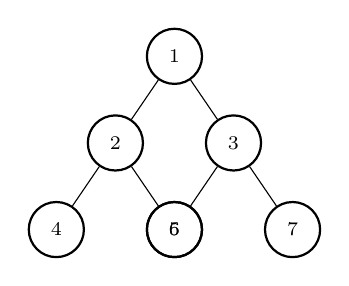
\begin{tikzpicture}[
  nodo/.style={draw=black, thick, circle, minimum size=7mm, font=\scriptsize},
  level distance=11mm, sibling distance=15mm
]
\node[nodo] {1}
  child { node[nodo] {2}
    child { node[nodo] {4} }
    child { node[nodo] {5} }
  }
  child { node[nodo] {3}
    child { node[nodo] {6} }
    child { node[nodo] {7} }
  };
\end{tikzpicture}

\small\textit{BFS: orden de expansión 1,2,3,4,5,6,7 (nivel por nivel).}
\end{minipage}
\hfill
\begin{minipage}{0.48\textwidth}
\centering
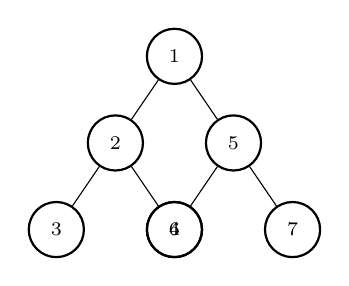
\begin{tikzpicture}[
  nodo/.style={draw=black, thick, circle, minimum size=7mm, font=\scriptsize},
  level distance=11mm, sibling distance=15mm
]
\node[nodo] {1}
  child { node[nodo] {2}
    child { node[nodo] {3} }
    child { node[nodo] {4} }
  }
  child { node[nodo] {5}
    child { node[nodo] {6} }
    child { node[nodo] {7} }
  };
\end{tikzpicture}

\small\textit{DFS: orden de expansión 1,2,3,4,5,6,7 (baja hasta el fondo antes de retroceder).}
\end{minipage}
\caption{Mismo árbol de búsqueda, dos órdenes de expansión distintos según la estructura de datos de la frontera
(cola FIFO en BFS, pila LIFO en DFS).}
\end{figure}

\subsection{Depth-Limited Search y Iterative Deepening (IDDFS)}

IDDFS ejecuta DFS con límite de profundidad creciente $l = 0, 1, 2, \ldots$

\begin{itemize}
    \item Combina las ventajas de BFS (completo, óptimo si costos iguales) con las de DFS (espacio lineal).
    \item Tiempo: $\bigO{b^d}$ \quad Espacio: $\bigO{bd}$
\end{itemize}

\subsection{Uniform-Cost Search (UCS)}

\begin{itemize}
    \item Expande el nodo con menor \textbf{costo de camino} $g(n)$ (cola de prioridad).
    \item Equivale a BFS cuando todos los costos son iguales.
    \item \textbf{Completo}: sí (si costos $> \epsilon > 0$).
    \item \textbf{Óptimo}: sí.
    \item Tiempo y espacio: $\bigO{b^{1+\lfloor C^*/\epsilon \rfloor}}$, donde $C^*$ es el costo óptimo.
\end{itemize}

\begin{example}[UCS sobre un grafo con costos]
    Usando el grafo de Rumania de la clase anterior, para ir de $Arad$ a $Bucarest$, UCS explora en este orden (por
    costo acumulado $g(n)$ creciente): $Arad(0)$, $Zerind(75)$, $Sibiu(140)$, $Oradea(146)$, $Rimnicu(220)$,
    $Fagaras(239)$, $Bucarest$ vía $Rimnicu \to Pitesti \to Bucarest$ con costo $418$, que resulta más barato que ir
    vía $Fagaras$ (costo $450$), aunque $Fagaras$ se alcance primero.
\end{example}

\subsection{Comparativa Búsqueda Desinformada}

\begin{center}
\begin{tabular}{lcccc}
\toprule
\textbf{Algoritmo} & \textbf{Completo} & \textbf{Óptimo} & \textbf{Tiempo} & \textbf{Espacio} \\
\midrule
BFS      & Sí & Sí* & $b^d$     & $b^d$ \\
DFS      & No & No  & $b^m$     & $bm$ \\
IDDFS    & Sí & Sí* & $b^d$     & $bd$ \\
UCS      & Sí & Sí  & $b^{C^*/\epsilon}$ & $b^{C^*/\epsilon}$ \\
\bottomrule
\multicolumn{5}{l}{\small *Óptimo si costos de paso son iguales}
\end{tabular}
\end{center}

% Clase 4 — Introducción a Búsqueda Informada
% Lectura: AIMA Sección 3.5
\section{Búsqueda Informada: Heurísticas}

\subsection{Función Heurística}

\begin{definition}[Heurística]
$h(n)$ es una función que estima el costo desde el nodo $n$ hasta la meta más cercana. Debe ser \textbf{admisible}: nunca sobreestima el costo real.
\end{definition}

\begin{remark}
Una heurística es \textbf{admisible} si $h(n) \leq h^*(n)$ para todo $n$, donde $h^*(n)$ es el costo real al llegar a la meta.
\end{remark}

\subsection{Greedy Best-First Search}

Expande el nodo que parece más cercano a la meta según $h(n)$.
\begin{itemize}
    \item Función de evaluación: $f(n) = h(n)$
    \item \textbf{No es óptimo} ni completo en general.
    \item Rápido en la práctica, puede quedar atrapado en mínimos locales.
\end{itemize}

\subsection{A*}

Combina el costo real del camino y la heurística:
$$f(n) = g(n) + h(n)$$

\begin{itemize}
    \item $g(n)$: costo del camino desde inicio hasta $n$
    \item $h(n)$: estimación del costo desde $n$ hasta la meta
    \item \textbf{Completo} y \textbf{óptimo} si $h$ es admisible (búsqueda en árbol) o consistente (búsqueda en grafo).
\end{itemize}

\begin{definition}[Consistencia / Monotonía]
$h$ es consistente si para todo nodo $n$ y sucesor $n'$:
$$h(n) \leq c(n, a, n') + h(n')$$
La consistencia implica admisibilidad.
\end{definition}

\begin{example}[Heurísticas comunes en una cuadrícula]
    Para un agente que se mueve en una cuadrícula 2D desde $(x_1,y_1)$ hasta $(x_2,y_2)$:
    \begin{itemize}
        \item \textbf{Distancia Manhattan}: $h(n) = |x_1-x_2| + |y_1-y_2|$. Admisible si el agente solo se mueve en
        horizontal/vertical (no sobreestima, porque es exactamente el número mínimo de pasos sin obstáculos).
        \item \textbf{Distancia euclidiana}: $h(n) = \sqrt{(x_1-x_2)^2 + (y_1-y_2)^2}$. Admisible si se permite
        movimiento diagonal, ya que nunca es mayor que el camino real.
    \end{itemize}
    Usar Manhattan cuando solo hay 4 movimientos posibles evita sobreestimar; usarla con movimiento diagonal
    permitido violaría la admisibilidad, porque el camino real podría ser más corto que la suma de catetos.
\end{example}

\begin{figure}[H]
\centering
\begin{tikzpicture}[
  nodo/.style={draw=black, thick, circle, minimum size=11mm, font=\scriptsize},
  descartado/.style={draw=black, thick, dashed, circle, minimum size=11mm, font=\scriptsize},
  meta/.style={draw=black, thick, double, circle, minimum size=11mm, font=\scriptsize}
]
\node[nodo] (arad)     at (0,0)    {\shortstack{A\\$g0,h366$}};
\node[nodo] (sibiu)    at (3,0.9)  {\shortstack{S\\$g140,h253$}};
\node[nodo] (zerind)   at (3,-0.9) {\shortstack{Z\\$g75,h374$}};
\node[nodo] (fagaras)  at (6,2.0)  {\shortstack{F\\$g239,h178$}};
\node[nodo] (rimnicu)  at (6,0.2)  {\shortstack{R\\$g220,h193$}};
\node[descartado] (bfagaras) at (9,2.0)  {\shortstack{B\\$g450,h0$}};
\node[nodo] (pitesti) at (9,0.2)  {\shortstack{P\\$g317,h100$}};
\node[meta] (bpitesti) at (12,0.2) {\shortstack{B\\$g418,h0$}};

\draw[-{Latex},thick] (arad) -- (sibiu);
\draw[-{Latex},thick] (arad) -- (zerind);
\draw[-{Latex},thick] (sibiu) -- (fagaras);
\draw[-{Latex},thick] (sibiu) -- (rimnicu);
\draw[-{Latex},thick,dashed] (fagaras) -- (bfagaras);
\draw[-{Latex},thick] (rimnicu) -- (pitesti);
\draw[-{Latex},thick] (pitesti) -- (bpitesti);
\end{tikzpicture}
\caption{Traza de A* sobre el mapa de Rumania (heurística: distancia en línea recta a Bucarest). A* siempre expande
el nodo de menor $f(n)=g(n)+h(n)$ de la frontera. Aunque Fagaras (F) llega primero a Bucarest con $f=450$ (nodo
punteado: se genera pero \textbf{se descarta}), Rimnicu (R) tiene $f=220+193=413$, menor que $f(F)=239+178=417$, así
que A* explora primero $R \to$ Pitesti (P) con $f=317+100=417$. Al final, la meta alcanzada por Pitesti tiene
$f=418$, menor que los $450$ de la rama de Fagaras, así que esa es la \textbf{solución óptima} (nodo de doble borde).}
\end{figure}



\chapter{Semana 2: Búsqueda Informada y Ambientes Complejos}

\begin{alertbox}[title=Eventos esta semana]
\begin{itemize}
    \item Publicación \textbf{Taller 1}
    \item \textbf{Examen 1} (al final de la semana)
\end{itemize}
\end{alertbox}

% Clase 1 — Búsqueda Informada Avanzada
% Lectura: AIMA Sección 3.6
\section{Búsqueda Informada Avanzada}

\subsection{Búsqueda con Memoria Acotada}

\subsubsection{Iterative Deepening A* (IDA*)}
Versión de A* que usa IDDFS con el valor de corte $f(n) = g(n) + h(n)$.
\begin{itemize}
    \item Espacio: $\bigO{bd}$
    \item Completo y óptimo (con $h$ admisible)
\end{itemize}

\subsubsection{Recursive Best-First Search (RBFS)}
Mantiene el mejor valor alternativo $f$ en cada nivel de recursión.
\begin{itemize}
    \item Espacio: $\bigO{bd}$
    \item Puede reexpandir nodos (regenera sub-árboles olvidados)
\end{itemize}

\subsubsection{SMA* (Simplified Memory-Bounded A*)}
Usa toda la memoria disponible; descarta el nodo con mayor $f$ cuando la memoria está llena.

\begin{figure}[H]
\centering
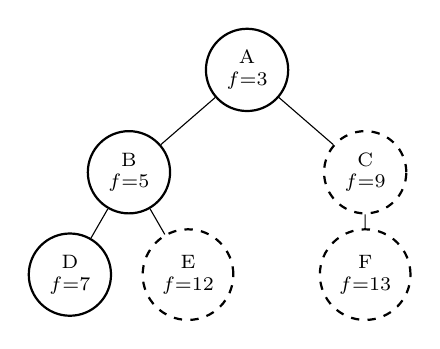
\begin{tikzpicture}[
  nodo/.style={draw=black, thick, circle, minimum size=8mm, font=\scriptsize},
  podado/.style={draw=black, thick, dashed, circle, minimum size=8mm, font=\scriptsize},
  level distance=13mm,
  level 1/.style={sibling distance=30mm},
  level 2/.style={sibling distance=15mm}
]
\node[nodo] {\shortstack{A\\$f{=}3$}}
  child { node[nodo] {\shortstack{B\\$f{=}5$}}
    child { node[nodo] {\shortstack{D\\$f{=}7$}} }
    child { node[podado] {\shortstack{E\\$f{=}12$}} }
  }
  child { node[podado] {\shortstack{C\\$f{=}9$}}
    child { node[podado] {\shortstack{F\\$f{=}13$}} }
  };
\end{tikzpicture}
\caption{IDA* con umbral inicial $f \leq 7$ (el valor de $h$ en la raíz): en la primera iteración se expanden $A$, $B$
y $D$ (todos con $f \leq 7$), y se podan $C$, $E$ y $F$ (nodos punteados, con $f > 7$). Si no se halla la meta, el
umbral sube al menor $f$ podado (aquí $9$) y se repite la búsqueda desde cero.}
\end{figure}

\subsection{Heurísticas: Dominancia y Creación}

\begin{definition}[Dominancia]
$h_2$ domina a $h_1$ si $h_2(n) \geq h_1(n)$ para todo $n$ y ambas son admisibles. Una heurística dominante expande menos nodos.
\end{definition}

Formas de construir heurísticas admisibles:
\begin{enumerate}
    \item \textbf{Relajación del problema}: eliminar restricciones del problema original.
    \item \textbf{Bases de datos de patrones}: precomputar costos exactos de subproblemas.
    \item \textbf{Máximo de heurísticas}: $h(n) = \max(h_1(n), h_2(n))$
\end{enumerate}

\begin{example}[8-puzzle: dos heurísticas admisibles]
    Sea $n$ un estado del 8-puzzle donde las fichas 1, 2 y 3 no están en su casilla objetivo.
    \begin{itemize}
        \item $h_1(n)$ = número de \textbf{fichas fuera de lugar}. Si 3 fichas están mal ubicadas, $h_1(n)=3$.
        \item $h_2(n)$ = suma de \textbf{distancias Manhattan} de cada ficha a su casilla objetivo. Si esas 3 fichas
        están, respectivamente, a 1, 2 y 3 movimientos de su lugar, $h_2(n) = 1+2+3 = 6$.
    \end{itemize}
    Ambas son admisibles (relajaciones del problema: $h_1$ ignora la restricción de que una ficha se mueva solo a una
    casilla adyacente vacía; $h_2$ ignora que solo puede moverse una ficha a la vez). Como $h_2(n) \geq h_1(n)$
    siempre, $h_2$ \textbf{domina} a $h_1$ y expande menos nodos en A*/IDA*.
\end{example}

% Clase 2 — Búsqueda en Ambientes Complejos
% Lectura: AIMA Cap. 4 (Hill Climbing + Algoritmos Genéticos)
\section{Búsqueda en Ambientes Complejos}

\subsection{Búsqueda Local}

A diferencia de la búsqueda sistemática, la búsqueda local opera sobre un \textbf{estado actual} sin mantener el camino recorrido. Útil cuando el objetivo es el estado mismo (no el camino).

\subsection{Hill Climbing (Ascenso de Colina)}

\begin{algorithm}[H]
\caption{Hill-Climbing}
\begin{algorithmic}[1]
\State $\text{current} \leftarrow \text{estado inicial}$
\Loop
    \State $\text{neighbor} \leftarrow$ mejor sucesor de $\text{current}$
    \If{$f(\text{neighbor}) \leq f(\text{current})$}
        \Return $\text{current}$
    \EndIf
    \State $\text{current} \leftarrow \text{neighbor}$
\EndLoop
\end{algorithmic}
\end{algorithm}

\textbf{Problemas}:
\begin{itemize}
    \item Máximos locales (no globales)
    \item Mesetas (\textit{plateaus}) y crestas
\end{itemize}

\textbf{Variantes}: Hill climbing estocástico, reinicio aleatorio, \textit{simulated annealing}.

\subsection{Simulated Annealing}

Permite movimientos malos con probabilidad $e^{\Delta E / T}$ donde $T$ decrece con el tiempo. Garantiza convergencia al óptimo global si $T$ baja suficientemente despacio.

\subsection{Algoritmos Genéticos}

Inspirados en la evolución biológica. Operan sobre una \textbf{población} de individuos (estados codificados como cadenas).

Operadores:
\begin{enumerate}
    \item \textbf{Selección}: individuos con mayor aptitud (\textit{fitness}) tienen más probabilidad de reproducirse.
    \item \textbf{Cruzamiento} (\textit{crossover}): combina dos individuos para producir descendencia.
    \item \textbf{Mutación}: cambia aleatoriamente genes con baja probabilidad.
\end{enumerate}

% Agrega aquí ejemplo del problema de las N-reinas con AG

% Clase 3 — Ejercicios de Búsqueda (preparación Examen 1)
% Referencia: Guía de Ejercicios IA Búsqueda
\section{Ejercicios de Búsqueda}

\begin{remark}
Esta clase es de ejercicios y repaso para el \textbf{Examen 1}.
Ver la \textit{Guía de Ejercicios: Búsqueda Desinformada e Informada}.
\end{remark}

\subsection{Guía de Ejercicios — Resumen de Bloques}

\subsubsection{Bloque 1: Agentes Inteligentes}
Caracterizar escenarios con PEAS, identificar tipo de agente y entorno.

\subsubsection{Bloque 2: Formulación de Problemas}
Definir estado inicial, modelo de transición, costo y test de meta para problemas concretos.

\subsubsection{Bloque 3: Búsqueda No Informada}
Aplicar BFS, DFS y UCS sobre grafos; analizar completitud y optimalidad.

\subsubsection{Bloque 4: Búsqueda Informada y Heurísticas}
Aplicar Greedy, A*, RBFS, SMA*; verificar admisibilidad y consistencia de heurísticas.

% ---- Espacio para soluciones de ejercicios ----

\begin{exercise}
Dado el grafo del Bloque 3 (Guía), aplica BFS, DFS y UCS.
Indica el orden de expansión y el camino solución encontrado.

\textbf{Solución:}
% ...
\end{exercise}



% =============================================
% PARTE 2: Razonamiento bajo Incertidumbre
% =============================================
\part{Razonamiento bajo Incertidumbre}

% =============================================
% SEMANA 3
% Temas: Búsqueda Adversaria y Juegos,
%        Razonamiento bajo Incertidumbre (Cap. 6, 12)
% Eventos: Entrega Taller 1
% =============================================
\chapter{Semana 3: Búsqueda Adversaria y Razonamiento bajo Incertidumbre}

\begin{alertbox}[title=Eventos esta semana]
\begin{itemize}
    \item \textbf{Entrega Taller 1}
\end{itemize}
\end{alertbox}

\section{Notas de Clase}

\subsection{Adversaria y juegos}

En cuanto a la agenda es:
\begin{enumerate}
    \item Teoría de juegos: como juegos de cero-suma
    \item Decisiones optimas en juegos: algoritmo minimax, decisiones optimas en juegos multijugador, podada alfa-beta
    \item Busqueda de arbol alpha-beta heuristico: funciones de eval, cortando la busqueda, podada forward
\end{enumerate}

Las \textbf{Relajación de restricciones} es una técnica utilizada para simplificar problemas complejos de busqueda y optimización. Consiste en \textit{eliminar o debilitar} algunas de las reglas de un problema para encontrar rapidamente una \textbf{solución aproximada}.
Los pasos son los siguientes:
\begin{itemize}
    \item saber definir las variables y los dominios de valores
    \item saber definir las restricciones entre variables
    \item conocer la forma de resolución de este tipo de problemas y posibles heuristicas
\end{itemize}

Un ejemplo claro es el del sudoku, en este caso hay 8 reinas(8 variables) cada una tiene su posición $(x,y)$ cuyo diminio entero representa su posición en la fila/columna $1..8$
Cada variable peude tener un \textbf{dominio distinto}
Las \textbf{restricciones} las reinas no pueden compartir fila ni columna ni diagonal. En el sudoku los numeros no pueden repetirse en filas ni columnas ni en bloques de 3x3.
Pueden involucrar a tantas variables como queramos (binarias, terniarias, etc)

\subsection{Como aborda un CSP?}
Generamos un espacio de busqueda, y analizamos cada variable/mejorar la complejidad:
Hay un conjunto de \textbf{heuríasticas} con distintas aproximaciones $(tecnicas de inferencia)$ y durante la busqueda \textit{propagración y consistencia} y \textit{criterios de ordenacion y seleccion de variables y valores a instanciar}

\textbf{Util} cuando tenemos un problema que se puede modelar como combinación de variables y restricciones.
$x_1$, $x_2$ $\in$ [1..10] donde $x_1$ + $x_2$ > 10 y  $x_1$ - $x_2$ < 5.
Nos interessa encontrar cualquier solución que satisfaga todas las restricciones - satisfactibilidad. Proceso de reolución my caro. Elevada explosión combinatoria de heuristicas.


Es una extensión y hay relajación de restricciones. 
Juegos estocasticos
Los juegos clásicos nosotros estamos viendo es si las maquinas peuden jugar? Puedan tomar mejores decisiones que nosotros?
Los juegos son simulaciones, ambientes parcialemnte observables, tiene un numero de estados bastante grandes.


\subsection{Procesos de decisión markovianas}
\subsection{Tipos de juegos}
Tipo de objetivos (First person S)
Hay distintos tipos de ejes:
\begin{itemize}
    \item Deterministico o estocasticos
    \item uno, dos o mas jugadores
\end{itemize}

\subsubsection{Juegos de cero suma}
Agentes tienen utilidades opuestas (valores en outcomes)
Se puede pensar en un valoe unico que uno maximiza y el otro minimiza

\begin{definition}
    Tenemos una utilidad que \textbf{U=A,B}, donde A maximiza y B minimiza
\end{definition}

\textit{Cooperación implicita}
En los juegos generales los agentes tienen utilidades independientes, cooperación indiferencia competencia -> posibles

Agente toma decisiones segun el punto de desición, la utilidad es como la recompensa

\subsection{Algoritmo MiniMax}
Se aplica para juegos deterministicos y de cero suma. Hay un arbol de espacio de estados. Jugador alterna turnos. Computa el valor minimax de cada nodo (Mejor Utilidad alcanzable contra un jugador racional)

Recompenssas $\neq$ Busqueda

U = $f(n)$ $g=$ camino recorrido y $h=$ heuristica

\subsubsection{Desiciones optimas en Juegos}

Casos de cooperación implicita, donde hay multiples jugadores se toma en cuenta el costo por accion y considerar que hace al agente adversario

\subsection{Limites de Recursos}
Son juego srealisticos no puede buscar a hojas
La solución es Depht-limiteed search, lo cual busca solucionar para un esapcio limitado, reemplazar las utilidades terminales con una funcion de evaluacion para posiciones no terminales
Podada Forward, uso de estadisticas. Algoritmo de corte probabilistico y reduccion de movimientos tardios


% =============================================
% SEMANA 4
% Temas: Redes Bayesianas, MDPs, CSP (Cap. 13, 16, 5)
% =============================================
\chapter{Semana 4: Redes Bayesianas, MDPs y CSP}

% Clase 1 — Redes Bayesianas
% Lectura: AIMA Cap. 13
\section{Redes Bayesianas}

\begin{definition}[Red Bayesiana]
Una red bayesiana es un grafo acíclico dirigido (DAG) donde:
\begin{itemize}
    \item Cada nodo representa una variable aleatoria.
    \item Los arcos representan dependencias directas.
    \item Cada nodo $X_i$ tiene una CPT: $P(X_i \mid \text{Parents}(X_i))$.
\end{itemize}
\end{definition}

\subsection{Semántica}

La distribución conjunta se factoriza como:
$$P(X_1, \ldots, X_n) = \prod_{i=1}^{n} P(X_i \mid \text{Parents}(X_i))$$

\subsection{Inferencia Exacta}

\begin{itemize}
    \item \textbf{Enumeración}: suma sobre todas las variables ocultas. Exponencial en el peor caso.
    \item \textbf{Eliminación de variables}: orden de eliminación importa para la eficiencia.
\end{itemize}

\subsection{Inferencia Aproximada}

\begin{itemize}
    \item \textbf{Muestreo directo}: muestrea según el orden topológico de la red.
    \item \textbf{Muestreo por rechazo}: descarta muestras inconsistentes con la evidencia.
    \item \textbf{Ponderación por verosimilitud}: fija la evidencia, pondera las muestras.
    \item \textbf{MCMC / Gibbs Sampling}: muestrea cada variable condicionada al resto.
\end{itemize}

\begin{example}[Red de alarma]
    Un sistema de alarma antirrobo se activa por un robo o (raramente) por un temblor. Dos vecinos, John y Mary,
    llaman si oyen la alarma, pero a veces confunden el teléfono con la alarma o no la oyen.
\end{example}

\begin{figure}[H]
\centering
\begin{tikzpicture}[
  var/.style={draw=black, thick, circle, minimum size=13mm, font=\small}
]
\node[var] (B) at (0,3)    {Robo};
\node[var] (E) at (4,3)    {Temblor};
\node[var] (A) at (2,1.2)  {Alarma};
\node[var] (J) at (0,-0.8) {John};
\node[var] (M) at (4,-0.8) {Mary};

\draw[-{Latex},thick] (B) -- (A);
\draw[-{Latex},thick] (E) -- (A);
\draw[-{Latex},thick] (A) -- (J);
\draw[-{Latex},thick] (A) -- (M);
\end{tikzpicture}
\caption{Red bayesiana Robo-Temblor-Alarma-John-Mary. Robo y Temblor son independientes a priori, pero se vuelven
\textbf{dependientes} al condicionar sobre Alarma (\textit{explaining away}); John y Mary son condicionalmente
independientes dado Alarma.}
\end{figure}

\begin{table}[H]
    \centering
    \begin{tabular}{cc}
        \toprule
        $P(\text{Robo})$ & $P(\text{Temblor})$ \\
        \midrule
        0.001 & 0.002 \\
        \bottomrule
    \end{tabular}
    \qquad
    \begin{tabular}{ccc}
        \toprule
        Robo & Temblor & $P(\text{Alarma})$ \\
        \midrule
        V & V & 0.95 \\
        V & F & 0.94 \\
        F & V & 0.29 \\
        F & F & 0.001 \\
        \bottomrule
    \end{tabular}
    \qquad
    \begin{tabular}{cc}
        \toprule
        Alarma & $P(\text{John})$ \\
        \midrule
        V & 0.90 \\
        F & 0.05 \\
        \bottomrule
    \end{tabular}
    \qquad
    \begin{tabular}{cc}
        \toprule
        Alarma & $P(\text{Mary})$ \\
        \midrule
        V & 0.70 \\
        F & 0.01 \\
        \bottomrule
    \end{tabular}
    \caption{CPTs de la red: la de Alarma tiene $2^2=4$ filas porque tiene 2 padres; John y Mary tienen 1 padre cada
    uno (Alarma), así que sus CPTs tienen 2 filas.}
\end{table}

% Clase 2 — Procesos de Decisión de Markov (MDPs)
% Lectura: AIMA Cap. 16
\section{Procesos de Decisión de Markov (MDPs)}

\begin{definition}[MDP]
Un MDP se define por la tupla $(S, A, P, R, \gamma)$:
\begin{itemize}
    \item $S$: conjunto de estados
    \item $A$: conjunto de acciones
    \item $P(s' \mid s, a)$: modelo de transición (probabilístico)
    \item $R(s, a, s')$: función de recompensa
    \item $\gamma \in [0, 1]$: factor de descuento
\end{itemize}
\end{definition}

\subsection{Propiedad de Markov}

$$P(s_{t+1} \mid s_t, a_t) = P(s_{t+1} \mid s_0, a_0, \ldots, s_t, a_t)$$

El futuro solo depende del estado presente, no del historial.

\subsection{Política y Utilidad}

\begin{itemize}
    \item \textbf{Política} $\pi(s)$: función que asigna una acción a cada estado.
    \item \textbf{Utilidad} (retorno descontado): $U = \sum_{t=0}^{\infty} \gamma^t R_t$
    \item \textbf{Política óptima} $\pi^*$: maximiza la utilidad esperada.
\end{itemize}

\subsection{Ecuación de Bellman}

$$U^*(s) = \max_a \sum_{s'} P(s' \mid s, a) \left[ R(s, a, s') + \gamma U^*(s') \right]$$

\subsection{Algoritmos de Solución}

\begin{itemize}
    \item \textbf{Value Iteration}: actualiza $U(s)$ iterativamente hasta convergencia.
    \item \textbf{Policy Iteration}: alterna entre evaluación de política y mejora de política.
\end{itemize}

% Agrega aquí ejemplo del mundo de cuadrículas (grid world)

% Clase 3 — Ejercicios de Razonamiento bajo Incertidumbre
\section{Ejercicios: Razonamiento bajo Incertidumbre}

\begin{notebox}
Repaso de probabilidad, redes bayesianas y MDPs.
\end{notebox}

% ---- Espacio para ejercicios en clase ----

\begin{exercise}
Dada la red bayesiana del ejemplo (Burglar-Earthquake-Alarm), calcula $P(\text{Burglary} \mid \text{JohnCalls} = T, \text{MaryCalls} = T)$ usando enumeración.

\textbf{Solución:}
% ...
\end{exercise}

% Clase 4 — Introducción a CSP
% Lectura: AIMA Cap. 5
\section{Problemas de Satisfacción de Restricciones (CSP)}

\begin{definition}[CSP]
Un CSP se define por:
\begin{itemize}
    \item $X = \{X_1, \ldots, X_n\}$: variables
    \item $D = \{D_1, \ldots, D_n\}$: dominios de cada variable
    \item $C$: conjunto de restricciones sobre subconjuntos de variables
\end{itemize}
La \textbf{solución} es una asignación completa y consistente.
\end{definition}

\subsection{Tipos de Restricciones}

\begin{itemize}
    \item \textbf{Unarias}: $X_i \in \{v_1, v_2\}$
    \item \textbf{Binarias}: $X_i \neq X_j$
    \item \textbf{Globales}: involucran más de 2 variables (ej. \texttt{AllDiff})
\end{itemize}

\subsection{Búsqueda con Retroceso (Backtracking)}

Asigna valores a variables una por una; retrocede cuando se viola una restricción.

\textbf{Heurísticas para mejorar el backtracking}:
\begin{enumerate}
    \item \textbf{MRV} (Minimum Remaining Values): elegir la variable con menos valores posibles.
    \item \textbf{Degree heuristic}: variable con más restricciones sobre variables no asignadas.
    \item \textbf{Least Constraining Value}: valor que deja más opciones para las demás variables.
\end{enumerate}

\begin{example}[Coloreado de un mapa]
    Cuatro regiones $W, X, Y, Z$ deben colorearse con $\{$rojo, verde, azul$\}$ de modo que regiones vecinas tengan
    colores distintos. Las adyacencias son: $W$-$X$, $W$-$Y$, $X$-$Y$, $X$-$Z$, $Y$-$Z$.
\end{example}

\begin{figure}[H]
\centering
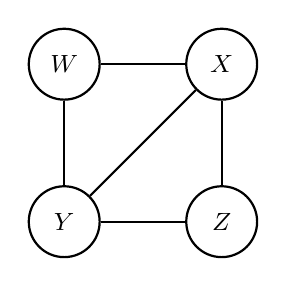
\begin{tikzpicture}[
  var/.style={draw=black, thick, circle, minimum size=9mm, font=\small}
]
\node[var] (W) at (0,2)   {$W$};
\node[var] (X) at (2,2)   {$X$};
\node[var] (Y) at (0,0)   {$Y$};
\node[var] (Z) at (2,0)   {$Z$};

\draw[thick] (W) -- (X);
\draw[thick] (W) -- (Y);
\draw[thick] (X) -- (Y);
\draw[thick] (X) -- (Z);
\draw[thick] (Y) -- (Z);
\end{tikzpicture}
\caption{Grafo de restricciones del CSP: cada nodo es una variable (región) y cada arista es una restricción binaria
de desigualdad con su vecina. $X$ y $Y$ tienen grado 3 (las más restringidas); son buenas candidatas para asignar
primero según la heurística de grado.}
\end{figure}


% =============================================
% SEMANA 5
% Temas: CSP avanzado, Agentes Lógicos (Cap. 5, 7)
% Eventos: Entrega Taller 2 | Examen 2
% =============================================
\chapter{Semana 5: CSP Avanzado y Agentes Lógicos}

\begin{alertbox}[title=Eventos esta semana]
\begin{itemize}
    \item \textbf{Entrega Taller 2}
    \item \textbf{Examen 2}
\end{itemize}
\end{alertbox}

\section{Problemas de Satisfacción de restricciones}

\subsection{Diagrama de Arbol}

En la clase anterior se definió un CSP como una tripla \textit{(variables, dominios, restricciones)} y se vió la \textbf{busqueda backtracking}, que es como un DFS + ordenamiento de variables + falla inmediata ante violación;
junto con dos mejoras clave:

\begin{itemize}
    \item \textbf{Filtrado} mediante $consistencia de arcos$; revisar si para cada valor de X, existe algún valor compatible en Y que detecta fallas inevitables antes que la simple revisión forward.
    \item \textbf{Ordenamiento} MRV \textit{(Minimun Remaining Values)} para variables y LCV \textit{(Least constraining value)} para valores 
\end{itemize}





% =============================================
% PARTE 3: Lógica y Representación del Conocimiento
% =============================================
\part{Lógica y Representación del Conocimiento}

% =============================================
% SEMANA 6
% Temas: Agentes Lógicos, Lógica de Primer Orden,
%        Inferencia (Cap. 7, 8, 9)
% =============================================
\chapter{Semana 6: Lógica y Representación del Conocimiento}

% Clase 1 — Agentes Lógicos: Inferencia Proposicional
% Lectura: AIMA Cap. 7
\section{Agentes Lógicos II: Inferencia Proposicional}

\subsection{Reglas de Inferencia}

\begin{tabular}{ll}
\toprule
\textbf{Regla} & \textbf{Forma} \\
\midrule
Modus Ponens & $\alpha \Rightarrow \beta,\ \alpha \vdash \beta$ \\
Modus Tollens & $\alpha \Rightarrow \beta,\ \neg\beta \vdash \neg\alpha$ \\
Resolución & $(\ell_1 \lor \cdots \lor \ell_k),\ (\neg\ell_1 \lor m_1 \lor \cdots) \vdash (m_1 \lor \cdots)$ \\
\bottomrule
\end{tabular}

\subsection{Resolución}

Algoritmo de inferencia completo para lógica proposicional en CNF:
\begin{enumerate}
    \item Convertir KB $\land \neg\alpha$ a CNF.
    \item Aplicar resolución hasta obtener la cláusula vacía (contradicción) o no poder seguir.
    \item Si se obtiene contradicción $\Rightarrow$ KB $\models \alpha$.
\end{enumerate}

\subsection{DPLL y WalkSAT}

\begin{itemize}
    \item \textbf{DPLL}: backtracking completo sobre asignaciones de verdad, con propagación de cláusulas unitarias.
    \item \textbf{WalkSAT}: búsqueda local incompleta, eficaz en la práctica para instancias satisfacibles.
\end{itemize}

\subsection{Ejemplo: Refutación por Resolución}

\begin{example}[Refutación]
    Sea $KB = \{P,\ P \Rightarrow Q,\ Q \Rightarrow R\}$ y se quiere probar $KB \models R$. Se convierte $KB \land \neg R$
    a CNF: $\{P,\ \neg P \lor Q,\ \neg Q \lor R,\ \neg R\}$, y se aplica resolución hasta obtener la cláusula vacía
    $\square$ (una contradicción), lo que confirma el entailment.
\end{example}

\begin{figure}[H]
\centering
\begin{tikzpicture}[
  clause/.style={draw=black, thick, rectangle, rounded corners=1pt, inner sep=4pt, font=\small}
]
\node[clause] (P)   at (0,0)      {$P$};
\node[clause] (PQ)  at (2.6,0)    {$\neg P \lor Q$};
\node[clause] (Q)   at (1.3,-1.4) {$Q$};

\node[clause] (QR)  at (4.2,-1.4) {$\neg Q \lor R$};
\node[clause] (R)   at (2.75,-2.8) {$R$};

\node[clause] (NR)  at (5.5,-2.8) {$\neg R$};
\node[clause] (NIL) at (4.1,-4.2) {$\square$};

\draw[-{Latex},thick] (P)  -- (Q);
\draw[-{Latex},thick] (PQ) -- (Q);
\draw[-{Latex},thick] (Q)  -- (R);
\draw[-{Latex},thick] (QR) -- (R);
\draw[-{Latex},thick] (R)  -- (NIL);
\draw[-{Latex},thick] (NR) -- (NIL);
\end{tikzpicture}
\caption{Árbol de refutación por resolución: cada nodo se obtiene combinando los dos que apuntan hacia él; llegar a la
cláusula vacía $\square$ demuestra que $KB \land \neg R$ es insatisfacible, es decir, $KB \models R$.}
\end{figure}

\begin{exercise}
    Sea $KB = \{A \lor B,\ \neg A \lor C,\ \neg B \lor C,\ \neg C \lor D\}$. Se quiere probar $KB \models D$ por
    refutación.
    \begin{enumerate}
        \item Escriba la cláusula que se agrega a $KB$ al negar la meta.
        \item Aplique resolución sobre $A \lor B$ y $\neg A \lor C$, y por separado sobre $\neg B \lor C$, para derivar
        una cláusula con únicamente $C$.
        \item Combine el resultado anterior con $\neg C \lor D$ y con la meta negada para llegar a la cláusula vacía.
        \item Dibuje el árbol de refutación completo, análogo al de la Figura anterior.
    \end{enumerate}
\end{exercise}


% Clase 2 — Lógica de Primer Orden
% Lectura: AIMA Cap. 8
\section{Lógica de Primer Orden (LPO)}

\subsection{Sintaxis}

Elementos de LPO:
\begin{itemize}
    \item \textbf{Constantes}: $Juan$, $UNIANDES$, \ldots
    \item \textbf{Variables}: $x, y, z, \ldots$
    \item \textbf{Predicados}: $Estudiante(x)$, $Mayor(x, y)$
    \item \textbf{Funciones}: $Padre(x)$, $Suma(x, y)$
    \item \textbf{Cuantificadores}: $\forall$ (universal), $\exists$ (existencial)
    \item \textbf{Conectivos}: $\neg, \land, \lor, \Rightarrow, \Leftrightarrow$
\end{itemize}

\subsection{Semántica}

Un \textbf{modelo} en LPO especifica:
\begin{itemize}
    \item El dominio de objetos
    \item La interpretación de constantes, predicados y funciones
\end{itemize}

\subsection{Cuantificadores}

$$\forall x\ P(x) \equiv \neg \exists x\ \neg P(x)$$
$$\exists x\ P(x) \equiv \neg \forall x\ \neg P(x)$$

\begin{remark}
$\forall x\ (P(x) \Rightarrow Q(x))$ es diferente de $\forall x\ (P(x) \land Q(x))$.
El cuantificador universal normalmente usa $\Rightarrow$; el existencial usa $\land$.
\end{remark}

\subsection{Ejemplo: Modelo en LPO}

\begin{example}[Modelo simple]
    Sea el dominio $D = \{\text{Juan}, \text{Maria}, \text{Pedro}\}$ y el predicado binario $Padre(x,y)$ ("$x$ es
    padre de $y$"). La interpretación de la Figura siguiente satisface $Padre(\text{Juan},\text{Maria})$ y
    $Padre(\text{Juan},\text{Pedro})$, y ninguna otra pareja.
\end{example}

\begin{figure}[H]
\centering
\begin{tikzpicture}[
  obj/.style={draw=black, thick, circle, minimum size=11mm, font=\small}
]
\node[obj] (juan)  at (0,0)   {Juan};
\node[obj] (maria) at (3.2,1) {Maria};
\node[obj] (pedro) at (3.2,-1){Pedro};

\draw[-{Latex},thick] (juan) -- node[above, font=\scriptsize]{$Padre$} (maria);
\draw[-{Latex},thick] (juan) -- node[below, font=\scriptsize]{$Padre$} (pedro);
\end{tikzpicture}
\caption{Modelo con dominio $\{\text{Juan},\text{Maria},\text{Pedro}\}$: cada flecha es una pareja $(x,y)$ para la
cual $Padre(x,y)$ es verdadero en este modelo. Cambiar las flechas cambia el modelo sin cambiar la sintaxis de la
oración.}
\end{figure}

\begin{exercise}
    Usando los predicados $Estudiante(x)$, $Curso(y)$, $Aprueba(x,y)$ y $Certificado(x,y)$, traduzca a LPO:
    \begin{enumerate}
        \item Todo estudiante que aprueba un curso recibe un certificado de ese curso.
        \item Existe al menos un estudiante que no ha aprobado ningún curso.
        \item Ningún estudiante aprueba todos los cursos.
    \end{enumerate}
    Para cada oración, indique si el cuantificador principal es $\forall$ o $\exists$ y justifique si el conectivo
    correcto dentro de su alcance es $\Rightarrow$ o $\land$.
\end{exercise}

% Clase 3 — LPO e Inferencia
% Lectura: AIMA Cap. 8-9
\section{LPO e Inferencia I}

\subsection{Bases de Conocimiento en LPO}

Las bases de conocimiento en LPO pueden expresar relaciones complejas de forma compacta, a diferencia de la lógica proposicional.

\subsection{Unificación}

Para aplicar reglas de inferencia en LPO se necesita \textbf{unificar} expresiones:

$$\text{UNIFY}(\alpha, \beta) = \theta \text{ tal que } \text{SUBST}(\theta, \alpha) = \text{SUBST}(\theta, \beta)$$

Algoritmo: recorre la estructura de ambas expresiones, construyendo sustituciones. Devuelve \textit{fallo} si no hay unificador.

\subsection{Inferencia con Cuantificadores}

\begin{itemize}
    \item \textbf{Instanciación universal}: $\forall x\ \alpha(x) \vdash \alpha(c)$ para cualquier constante $c$.
    \item \textbf{Instanciación existencial}: $\exists x\ \alpha(x) \vdash \alpha(k)$ donde $k$ es una nueva constante de Skolem.
    \item \textbf{Skolemización}: eliminar cuantificadores existenciales introduciendo constantes/funciones de Skolem.
\end{itemize}

\subsection{Forma Normal de Clausura (CNF en LPO)}

Pasos para convertir a CNF:
\begin{enumerate}
    \item Eliminar bicondicionales e implicaciones.
    \item Mover $\neg$ hacia adentro (De Morgan, reglas de cuantificadores).
    \item Estandarizar variables.
    \item Skolemizar.
    \item Eliminar cuantificadores universales.
    \item Distribuir $\lor$ sobre $\land$.
\end{enumerate}

% Clase 4 — Inferencia en LPO
% Lectura: AIMA Cap. 9
\section{Inferencia en LPO II}

\subsection{Encadenamiento hacia adelante (Forward Chaining)}

Aplica reglas de la forma $P_1 \land \cdots \land P_n \Rightarrow Q$ para derivar nuevos hechos hasta alcanzar la meta.
\begin{itemize}
    \item Completo para bases de conocimiento de \textbf{cláusulas de Horn}.
    \item Dirigido por los datos.
\end{itemize}

\subsection{Encadenamiento hacia atrás (Backward Chaining)}

Parte de la meta y trabaja hacia atrás buscando hechos o submetas.
\begin{itemize}
    \item Completo para cláusulas de Horn.
    \item Base de Prolog.
    \item Puede ciclar si no se controla.
\end{itemize}

\subsection{Resolución en LPO}

Generaliza la resolución proposicional usando unificación:

$$\frac{\ell_1 \lor \cdots \lor \ell_k \quad \neg m_1 \lor \cdots \lor \neg m_j}{\text{SUBST}(\theta, \ell_1 \lor \cdots \lor m_j)}$$

donde $\theta = \text{UNIFY}(\ell_i, m_k)$.

\begin{itemize}
    \item \textbf{Refutación por resolución}: completa para LPO (Teorema de Completitud de Gödel).
\end{itemize}

% Agrega aquí ejemplos de encadenamiento y resolución


% Clase 5 — Ejercicios resueltos: Guía de Agentes Lógicos (completa)
\section{Ejercicios: Guía de Agentes Lógicos (con solución paso a paso)}

Esta sección resuelve, de principio a fin, la \textit{Guía de Ejercicios: Agentes Lógicos}. Cada
respuesta se justifica explícitamente; en los casos falsos se da la versión corregida, y en los
casos de tablas de verdad o resolución se muestra cada paso.

\subsection{Bloque 1: Conceptos Fundamentales de Agentes Lógicos}

\paragraph{Parte A --- Consecuencia Lógica y Modelos}

\begin{enumerate}
    \item \textit{``Una base de conocimiento KB implica lógicamente una sentencia $\alpha$ (escrito
    $KB \models \alpha$) si y solo si $\alpha$ es verdadera en todo modelo en el que KB es
    verdadera.''}\\
    \textbf{Verdadero.} Es exactamente la definición semántica de consecuencia lógica: un modelo de
    KB es una interpretación donde toda sentencia de KB es verdadera, y $KB \models \alpha$ exige que
    $\alpha$ también lo sea en \emph{todos} esos modelos.

    \item \textit{``Si $KB \models \alpha$, entonces $\alpha$ debe ser verdadera en todos los mundos
    posibles, sin importar lo que diga KB.''}\\
    \textbf{Falso.} $\alpha$ solo tiene que ser verdadera en los modelos donde \emph{KB también es
    verdadera}; en los modelos donde KB es falsa, $\alpha$ puede ser falsa sin violar $KB \models
    \alpha$.\\
    \textbf{Corrección:} Si $KB \models \alpha$, entonces $\alpha$ es verdadera en todo modelo en el
    que KB es verdadera (no en todo modelo posible sin restricción).

    \item \textit{``Una sentencia es válida (tautología) si es verdadera en algunos los modelos
    posibles.''}\\
    \textbf{Falso.} Eso describe \emph{satisfacibilidad}, no validez.\\
    \textbf{Corrección:} Una sentencia es válida (tautología) si es verdadera en \textbf{todos} los
    modelos posibles.

    \item \textit{``Una sentencia es satisfacible si existe al menos un modelo en el que es
    verdadera.''}\\
    \textbf{Verdadero.} Es la definición estándar de satisfacibilidad.

    \item \textit{``Si una sentencia es insatisfacible, entonces su negación es satisficible.''}\\
    \textbf{Verdadero.} Si $\alpha$ es insatisfacible, es falsa en todo modelo, por lo tanto $\neg
    \alpha$ es verdadera en todo modelo (es decir, $\neg\alpha$ es válida). Toda sentencia válida es,
    en particular, satisfacible (verdadera en al menos un modelo: todos ellos).
\end{enumerate}

\paragraph{Parte B --- Algoritmos de Inferencia y Verificación de Modelos}

\begin{enumerate}
    \item \textit{``El algoritmo TT-Implica? enumera todos los modelos posibles para verificar si
    $KB \models \alpha$, siendo correcto y completo pero exponencial en el número de símbolos.''}\\
    \textbf{Verdadero.} Con $n$ símbolos proposicionales hay $2^n$ asignaciones de verdad posibles;
    TT-Implica? las recorre todas, por lo que es $\bigO{2^n}$, pero al ser una enumeración exhaustiva
    es correcto (sound) y completo.

    \item \textit{``Un procedimiento de prueba es correcto (sound) si sólo deriva sentencias que son
    consecuencia lógica de KB.''}\\
    \textbf{Verdadero.} Esa es la definición de \textit{soundness}: nunca deriva una sentencia falsa
    a partir de premisas verdaderas. (La \textit{completitud} es la propiedad complementaria: deriva
    \emph{todas} las sentencias que son consecuencia lógica.)

    \item \textit{``Modus Ponens establece: si $\alpha \Rightarrow \beta$ está en KB, y $\beta$ es
    verdadera, entonces podemos inferir $\alpha$.''}\\
    \textbf{Falso.} Esto es la falacia de \textit{afirmar el consecuente}, una regla inválida.\\
    \textbf{Corrección:} Modus Ponens establece que si $\alpha \Rightarrow \beta$ está en KB y
    $\alpha$ es verdadera, entonces podemos inferir $\beta$.

    \item \textit{``La regla de resolución establece que de las cláusulas $(\ell_1 \lor \cdots \lor
    \ell_k \lor m)$ y $(\neg m \lor n_1 \lor \cdots \lor n_j)$ se puede derivar $(\ell_1 \lor \cdots
    \lor \ell_k \lor n_1 \lor \cdots \lor n_j)$.''}\\
    \textbf{Verdadero.} Es exactamente la regla de resolución binaria: se cancela el par
    complementario $m / \neg m$ y se unen el resto de los literales de ambas cláusulas.

    \item \textit{``El algoritmo DPLL es una mejora sobre la enumeración básica de tablas de verdad
    para verificar satisfacibilidad.''}\\
    \textbf{Verdadero.} DPLL añade propagación de cláusulas unitarias, eliminación de literales puros
    y poda temprana (\textit{early termination}) sobre el backtracking de fuerza bruta, evitando
    explorar ramas completas del árbol de asignaciones cuando ya se sabe que fallarán.

    \item \textit{``El encadenamiento hacia adelante está orientado a metas: trabaja hacia atrás
    desde una consulta para determinar si KB la soporta.''}\\
    \textbf{Falso.} Esa descripción corresponde al encadenamiento \textbf{hacia atrás}.\\
    \textbf{Corrección:} El encadenamiento hacia adelante está orientado a \textbf{datos}: parte de
    los hechos conocidos en KB y dispara reglas repetidamente hasta derivar la consulta (o hasta que
    no se puedan agregar más hechos).
\end{enumerate}

\paragraph{Parte C --- Reglas de Inferencia}

\begin{enumerate}
    \item De $(P \Rightarrow Q)$ y $P$, concluir $Q$.\\
    \textbf{Nombre:} Modus Ponens. \quad \textbf{Válida:} Sí. Si $P\Rightarrow Q$ es verdadera y $P$
    es verdadera, la única fila de la tabla de verdad compatible con $P\Rightarrow Q$ verdadera y $P$
    verdadera tiene $Q$ verdadera.

    \item De $(P \Rightarrow Q)$ y $\neg Q$, concluir $\neg P$.\\
    \textbf{Nombre:} Modus Tollens. \quad \textbf{Válida:} Sí. Si $P$ fuera verdadera, $P\Rightarrow
    Q$ obligaría a $Q$ verdadera, contradiciendo $\neg Q$; por lo tanto $P$ debe ser falsa.

    \item De $P$ y $Q$, concluir $(P \land Q)$.\\
    \textbf{Nombre:} Introducción de la conjunción (And-Introduction). \quad \textbf{Válida:} Sí, por
    definición de $\land$.

    \item De $(P \lor Q)$ y $\neg P$, concluir $Q$.\\
    \textbf{Nombre:} Silogismo disyuntivo (resolución unitaria). \quad \textbf{Válida:} Sí. Como $P$
    es falsa, para que $P\lor Q$ sea verdadera, $Q$ debe serlo.

    \item De $(P \Rightarrow Q)$ y $(Q \Rightarrow R)$, concluir $(P \Rightarrow R)$.\\
    \textbf{Nombre:} Silogismo hipotético (transitividad de la implicación). \quad \textbf{Válida:}
    Sí (se demuestra formalmente en el Bloque 4, Problema 4.1.3, convirtiendo la sentencia a FNC).

    \item De $(P \Rightarrow Q)$ y $\neg P$, concluir $\neg Q$.\\
    \textbf{Nombre:} Negación del antecedente (falacia). \quad \textbf{Válida:} No, es \textbf{inválida}.
    \textbf{Contraejemplo:} $P = F$, $Q = T$: $P\Rightarrow Q$ es verdadera y $\neg P$ es verdadera,
    pero $\neg Q$ es falsa.
\end{enumerate}

\subsection{Bloque 2: Validez y Satisfacibilidad}

\paragraph{Problema 2.1 --- Validez y Satisfacibilidad (Ej. 13, Cap. 7 AIMA)}

\begin{enumerate}
    \item $Humo \Rightarrow Humo$.\\
    \begin{tabular}{cc}
        \toprule
        $Humo$ & $Humo\Rightarrow Humo$ \\
        \midrule
        T & T \\
        F & T \\
        \bottomrule
    \end{tabular}\\
    Todas las filas son verdaderas $\Rightarrow$ \textbf{Válida} (instancia del esquema $\alpha
    \Rightarrow \alpha$, siempre tautológico).

    \item $Humo \Rightarrow Fuego$.\\
    \begin{tabular}{ccc}
        \toprule
        $Humo$ & $Fuego$ & $Humo\Rightarrow Fuego$ \\
        \midrule
        T & T & T \\
        T & F & F \\
        F & T & T \\
        F & F & T \\
        \bottomrule
    \end{tabular}\\
    Hay filas verdaderas y una falsa $\Rightarrow$ \textbf{Satisfacible, pero no válida} (contingente).

    \item $(Humo \Rightarrow Fuego) \Rightarrow (\neg Humo \Rightarrow \neg Fuego)$.\\
    \begin{tabular}{cccccc}
        \toprule
        $Humo$ & $Fuego$ & $H\Rightarrow F$ & $\neg H$ & $\neg F$ & $(H\Rightarrow F)\Rightarrow(\neg H\Rightarrow\neg F)$ \\
        \midrule
        T & T & T & F & F & T \\
        T & F & F & F & T & T \\
        F & T & T & T & F & \textbf{F} \\
        F & F & T & T & T & T \\
        \bottomrule
    \end{tabular}\\
    La fila $Humo=F, Fuego=T$ da Falso, y las demás dan Verdadero $\Rightarrow$
    \textbf{Satisfacible, pero no válida} (contingente).

    \item $Humo \lor Fuego \lor \neg Fuego$.\\
    El subtérmino $Fuego \lor \neg Fuego$ ya es una tautología (verdadero sin importar el valor de
    $Fuego$), así que toda la disyunción es verdadera en las 4 filas posibles de $(Humo,Fuego)$
    $\Rightarrow$ \textbf{Válida}.

    \item $((Humo \land Calor) \Rightarrow Fuego) \Leftrightarrow ((Humo \Rightarrow Fuego) \lor
    (Calor \Rightarrow Fuego))$.\\
    \begin{tabular}{ccccccccc}
        \toprule
        $H$ & $C$ & $Fu$ & $H\land C$ & $A=(H\land C)\Rightarrow Fu$ & $H\Rightarrow Fu$ & $C\Rightarrow Fu$ & $B$ (su OR) & $A\Leftrightarrow B$\\
        \midrule
        T&T&T&T&T&T&T&T&T\\
        T&T&F&T&F&F&F&F&T\\
        T&F&T&F&T&T&T&T&T\\
        T&F&F&F&T&F&T&T&T\\
        F&T&T&F&T&T&T&T&T\\
        F&T&F&F&T&T&F&T&T\\
        F&F&T&F&T&T&T&T&T\\
        F&F&F&F&T&T&T&T&T\\
        \bottomrule
    \end{tabular}\\
    Las 8 filas dan Verdadero $\Rightarrow$ \textbf{Válida}. (Se puede confirmar algebraicamente:
    $(H\land C)\Rightarrow Fu \equiv \neg H \lor \neg C \lor Fu$, y $(H\Rightarrow Fu)\lor(C\Rightarrow
    Fu) \equiv (\neg H\lor Fu)\lor(\neg C\lor Fu) \equiv \neg H\lor\neg C\lor Fu$: ambos lados son
    \emph{idénticos}, por lo que el bicondicional es una tautología.)
\end{enumerate}

\paragraph{Problema 2.2 --- Verificación de Consecuencia Lógica}

\begin{enumerate}
    \item $A \Leftrightarrow B \models \neg A \lor B$?\\
    \begin{tabular}{cccc}
        \toprule
        $A$ & $B$ & $A\Leftrightarrow B$ & $\neg A \lor B$ \\
        \midrule
        T & T & T & T \\
        T & F & F & F \\
        F & T & F & T \\
        F & F & T & T \\
        \bottomrule
    \end{tabular}\\
    En las dos filas donde $A\Leftrightarrow B$ es verdadera (fila 1 y fila 4), $\neg A \lor B$
    también lo es. \textbf{Correcta.} Justificación algebraica: $A\Leftrightarrow B \equiv (A
    \Rightarrow B)\land(B\Rightarrow A)$, y $A\Rightarrow B \equiv \neg A \lor B$; por lo tanto
    $A\Leftrightarrow B$ implica cada uno de sus conjuntos, en particular $\neg A \lor B$.

    \item $(A \lor B) \land (\neg C \lor \neg D \lor E) \models (A \lor B)$?\\
    \textbf{Correcta}, y de forma trivial: cualquier modelo que satisface una conjunción $X \land Y$
    satisface, en particular, cada conjunto por separado ($X$ e $Y$); aquí $X = (A\lor B)$. No hace
    falta enumerar las $2^5=32$ filas: es una instancia directa de la regla de \textit{eliminación de
    la conjunción} ($X \land Y \models X$), válida para cualquier $X, Y$.

    \item $(A \lor B) \land (\neg C \lor \neg D \lor E) \models (A \lor B) \land (\neg D \lor E)$?\\
    \textbf{No es correcta.} Contraejemplo: $A=T,\ B=F,\ C=F,\ D=T,\ E=F$.\\
    Verificación paso a paso:
    \begin{itemize}
        \item $A \lor B = T \lor F = T$.
        \item $\neg C \lor \neg D \lor E = \neg F \lor \neg T \lor F = T \lor F \lor F = T$.
        \item Lado izquierdo (premisa) $= T \land T = T$: el modelo satisface la premisa.
        \item $\neg D \lor E = \neg T \lor F = F \lor F = F$.
        \item Lado derecho (conclusión) $= (A\lor B) \land (\neg D \lor E) = T \land F = F$.
    \end{itemize}
    La premisa es verdadera y la conclusión es falsa en este modelo, así que la premisa \textbf{no}
    implica la conclusión. El error es que $\neg C \lor \neg D \lor E$ puede ser verdadera "gracias a"
    $\neg C$ sin decir nada sobre $\neg D \lor E$.
\end{enumerate}

\subsection{Bloque 3: Modelamiento de Lenguaje Natural — El Problema de la Mansión Embrujada}

\paragraph{Parte A --- Definición de Símbolos Proposicionales}

Además de $F_{x,y}$, $T_{x,y}$, $Frio_{x,y}$ y $Crujido_{x,y}$ (dados en el enunciado), se necesitan
símbolos para registrar el estado epistémico del robot:
\begin{itemize}
    \item $Segura_{x,y}$ = ``El robot ha \emph{probado} que la habitación $(x,y)$ es segura (no tiene
    Fantasma ni Trampa)''.
    \item $Visitada_{x,y}$ = ``El robot ya visitó la habitación $(x,y)$''.
\end{itemize}

\paragraph{Parte B --- Codificación de las Reglas}

\begin{enumerate}
    \item La entrada es segura:
    \[
        \neg F_{1,1} \land \neg T_{1,1}
    \]

    \item Frío en $(1,1)$ implica Fantasma en una adyacente:
    \[
        Frio_{1,1} \Leftrightarrow (F_{2,1} \lor F_{1,2})
    \]

    \item Crujido en $(1,1)$ implica Trampa en una adyacente:
    \[
        Crujido_{1,1} \Leftrightarrow (T_{2,1} \lor T_{1,2})
    \]

    \item Axioma de Frío para $(2,2)$, adyacente a $(1,2)$, $(3,2)$ y $(2,1)$:
    \[
        Frio_{2,2} \Leftrightarrow (F_{1,2} \lor F_{3,2} \lor F_{2,1})
    \]

    \item A lo sumo un Fantasma en toda la mansión (6 habitaciones: $(1,1)$ a $(3,2)$). Usando
    implicaciones, se afirma que si una habitación tiene el Fantasma, \textbf{ninguna otra} lo tiene:
    \[
        \bigwedge_{(x,y) \neq (x',y')} \big(F_{x,y} \Rightarrow \neg F_{x',y'}\big)
    \]
    Por ejemplo, para $(1,1)$:
    \[
        F_{1,1} \Rightarrow (\neg F_{2,1} \land \neg F_{3,1} \land \neg F_{1,2} \land \neg F_{2,2}
        \land \neg F_{3,2})
    \]
    y una implicación análoga se escribe partiendo de cada una de las otras 5 habitaciones (en total
    $\binom{6}{2}=15$ pares de restricción, cada uno equivalente a la cláusula $\neg F_{x,y} \lor
    \neg F_{x',y'}$).
\end{enumerate}

\paragraph{Parte C --- Razonamiento a partir de las Percepciones}

Adyacencias en la cuadrícula $3\times2$: $(1,1)$--$(2,1)$--$(3,1)$ (fila inferior) y $(1,2)$--$(2,2)$--$(3,2)$
(fila superior), con $(1,1)$--$(1,2)$, $(2,1)$--$(2,2)$ y $(3,1)$--$(3,2)$ uniendo las dos filas.

\begin{enumerate}
    \item \textbf{¿Puede el robot concluir que $(2,2)$ contiene una Trampa?}\\
    \textbf{Razonamiento (paso a paso):}
    \begin{enumerate}
        \item En $(1,1)$ el robot percibe ``Sin Crujido''. Por el axioma de la Parte B, ítem 3,
        $Crujido_{1,1} \Leftrightarrow (T_{2,1}\lor T_{1,2})$; como $Crujido_{1,1}$ es falso, se
        concluye $\neg T_{2,1} \land \neg T_{1,2}$ (ni $(2,1)$ ni $(1,2)$ tienen Trampa). Junto con
        $\neg F_{2,1}\land\neg F_{1,2}$ (del axioma de Frío) y la entrada segura, esto confirma que
        $(2,1)$ y $(1,2)$ son seguras — de ahí que el robot pudiera moverse a ambas.
        \item El axioma de Crujido para $(1,2)$ (adyacente a $(1,1)$ y $(2,2)$) es:
        \[
            Crujido_{1,2} \Leftrightarrow (T_{1,1} \lor T_{2,2})
        \]
        \item El robot percibe Crujido en $(1,2)$, luego $Crujido_{1,2}$ es verdadero, así que
        $T_{1,1} \lor T_{2,2}$ es verdadero (Modus Ponens sobre el bicondicional).
        \item Se sabe que $\neg T_{1,1}$ (la entrada es segura, Parte B ítem 1).
        \item Por silogismo disyuntivo sobre $T_{1,1} \lor T_{2,2}$ y $\neg T_{1,1}$, se concluye
        $T_{2,2}$.
    \end{enumerate}
    \textbf{Conclusión:} \textbf{Sí}, el robot puede concluir con certeza que hay una Trampa en
    $(2,2)$.

    \item \textbf{¿Puede el robot concluir que $(3,1)$ es segura para entrar?}\\
    \textbf{Razonamiento (paso a paso):}
    \begin{enumerate}
        \item $(3,1)$ es adyacente a $(2,1)$ y $(3,2)$. El robot solo tiene percepciones en $(1,1)$,
        $(2,1)$ y $(1,2)$; nunca ha estado en $(3,2)$, así que no hay información directa sobre esa
        adyacencia.
        \item En $(2,1)$ el robot solo percibió Crujido (no Frío). Por el axioma de Frío para
        $(2,1)$: $Frio_{2,1} \Leftrightarrow (F_{1,1}\lor F_{3,1}\lor F_{2,2})$. Como $Frio_{2,1}$ es
        falso, se concluye $\neg F_{1,1} \land \neg F_{3,1} \land \neg F_{2,2}$: en particular
        $\neg F_{3,1}$ (no hay Fantasma en $(3,1)$).
        \item Por el axioma de Crujido para $(2,1)$: $Crujido_{2,1} \Leftrightarrow (T_{1,1}\lor
        T_{3,1}\lor T_{2,2})$. Como $Crujido_{2,1}$ es verdadero y $\neg T_{1,1}$ (entrada segura),
        se obtiene $T_{3,1}\lor T_{2,2}$.
        \item Del ítem anterior de este mismo bloque ya se sabe $T_{2,2}$ es verdadero. Esto por sí
        solo \textbf{ya satisface} la disyunción $T_{3,1}\lor T_{2,2}$, sin necesidad de que $T_{3,1}$
        sea verdadero. Es decir, la KB \emph{no fuerza} un valor de verdad para $T_{3,1}$: es
        consistente tanto con $T_{3,1}=Verdadero$ como con $T_{3,1}=Falso$.
    \end{enumerate}
    \textbf{Conclusión:} \textbf{No.} Aunque se sabe que $(3,1)$ no tiene Fantasma ($\neg F_{3,1}$),
    el estado de la Trampa en $(3,1)$ queda \textbf{indeterminado} (el Crujido percibido en $(2,1)$ ya
    queda explicado por la Trampa en $(2,2)$). Como la seguridad exige certeza sobre \emph{ambos}
    peligros, el robot no puede probar que $(3,1)$ sea segura y, según la regla del enunciado, no
    puede entrar todavía.
\end{enumerate}

\subsection{Bloque 4: Conversión a FNC y Resolución}

\paragraph{Problema 4.1 --- Conversión a FNC}

\begin{enumerate}
    \item $P \Leftrightarrow Q$\\
    \textbf{Paso a paso:}
    \begin{align*}
        P \Leftrightarrow Q &\equiv (P \Rightarrow Q) \land (Q \Rightarrow P) &&\text{(def. de }\Leftrightarrow\text{)}\\
        &\equiv (\neg P \lor Q) \land (\neg Q \lor P) &&\text{(eliminar }\Rightarrow\text{)}
    \end{align*}
    Ya es conjunción de disyunciones de literales: no hace falta distribuir más.\\
    \textbf{FNC:} $(\neg P \lor Q) \land (\neg Q \lor P)$

    \item $\neg(P \lor Q) \Rightarrow R$\\
    \textbf{Paso a paso:}
    \begin{align*}
        \neg(P\lor Q) \Rightarrow R &\equiv \neg\neg(P\lor Q) \lor R &&\text{(eliminar }\Rightarrow\text{)}\\
        &\equiv (P \lor Q) \lor R &&\text{(doble negación)}\\
        &\equiv P \lor Q \lor R &&\text{(ya es una sola cláusula)}
    \end{align*}
    \textbf{FNC:} $P \lor Q \lor R$

    \item $(A \Rightarrow B) \land (B \Rightarrow C) \Rightarrow (A \Rightarrow C)$\\
    \textbf{Paso a paso:}
    \begin{align*}
        &\equiv \neg\big[(\neg A \lor B)\land(\neg B \lor C)\big] \lor (\neg A \lor C)
        &&\text{(eliminar las tres }\Rightarrow\text{)}\\
        &\equiv \big[\neg(\neg A\lor B) \lor \neg(\neg B\lor C)\big] \lor (\neg A \lor C)
        &&\text{(De Morgan)}\\
        &\equiv (A \land \neg B) \lor (B \land \neg C) \lor \neg A \lor C
        &&\text{(De Morgan otra vez, doble negación)}
    \end{align*}
    Distribuir $\lor$ sobre $\land$, primero $(A\land\neg B)\lor(B\land\neg C)$:
    \[
        (A\lor B)\land(A\lor\neg C)\land(\neg B\lor B)\land(\neg B\lor\neg C)
    \]
    Como $\neg B \lor B$ es tautología, se elimina esa cláusula (no aporta restricción):
    \[
        (A\lor B)\land(A\lor\neg C)\land(\neg B\lor\neg C)
    \]
    Ahora se distribuye ese resultado con $\lor\ (\neg A \lor C)$, clausula por clausula:
    \begin{align*}
        (A\lor B\lor\neg A\lor C) \;&\land\; (A\lor\neg C\lor\neg A\lor C) \;\land\; (\neg B\lor\neg C\lor\neg A\lor C)
    \end{align*}
    Cada una de las tres cláusulas contiene un literal y su negación ($A,\neg A$ en la primera y
    segunda; $C,\neg C$ en la segunda y tercera), por lo que \textbf{las tres son tautológicas} y se
    pueden eliminar todas.\\
    \textbf{Respuesta:} La FNC resultante no tiene cláusulas (todas son tautologías), lo cual
    significa que la sentencia original es verdadera en \emph{todo} modelo: es una \textbf{validez}
    (el silogismo hipotético / transitividad de la implicación, coherente con la Parte C, ítem 5, del
    Bloque 1).\\
    \textbf{FNC:} $\top$ (conjunción vacía de cláusulas, todas tautológicas)
\end{enumerate}

\paragraph{Problema 4.2 --- Validez, FNC y Prueba por Resolución (Ej. 13, Cap. 7 AIMA)}

Sentencia: $[(Comida \Rightarrow Fiesta) \lor (Bebidas \Rightarrow Fiesta)] \Rightarrow [(Comida
\land Bebidas) \Rightarrow Fiesta]$. Se abrevia $Co=Comida$, $Be=Bebidas$, $Fi=Fiesta$.

\begin{enumerate}
    \item \textbf{Clasificación por enumeración:}\\
    \begin{tabular}{ccc|ccc|cc|c}
        \toprule
        $Co$ & $Be$ & $Fi$ & $Co{\Rightarrow}Fi$ & $Be{\Rightarrow}Fi$ & LHS(or) & $Co{\land}Be$ & RHS & Total \\
        \midrule
        T&T&T&T&T&T&T&T&T\\
        T&T&F&F&F&F&T&F&T\\
        T&F&T&T&T&T&F&T&T\\
        T&F&F&F&T&T&F&T&T\\
        F&T&T&T&T&T&F&T&T\\
        F&T&F&T&F&T&F&T&T\\
        F&F&T&T&T&T&F&T&T\\
        F&F&F&T&T&T&F&T&T\\
        \bottomrule
    \end{tabular}\\
    \textbf{Clasificación:} \textbf{Válida.}\\
    \textbf{Justificación:} Las 8 filas dan verdadero. Es interesante notar que la única fila en la
    que el consecuente (RHS) es falso es $Co{=}T,Be{=}T,Fi{=}F$; pero en esa misma fila el antecedente
    (LHS) también es falso, así que la implicación completa es $F\Rightarrow F = T$.

    \item \textbf{FNC de cada lado:}\\
    \textbf{FNC lado izquierdo:}
    \begin{align*}
        (Co\Rightarrow Fi)\lor(Be\Rightarrow Fi) &\equiv (\neg Co\lor Fi)\lor(\neg Be\lor Fi)
        &&\text{(eliminar }\Rightarrow\text{)}\\
        &\equiv \neg Co \lor \neg Be \lor Fi &&\text{(ya es una sola cláusula; $Fi$ se repite)}
    \end{align*}
    \textbf{FNC lado izquierdo:} $\neg Co \lor \neg Be \lor Fi$

    \textbf{FNC lado derecho:}
    \begin{align*}
        (Co\land Be)\Rightarrow Fi &\equiv \neg(Co\land Be)\lor Fi &&\text{(eliminar }\Rightarrow\text{)}\\
        &\equiv \neg Co\lor\neg Be\lor Fi &&\text{(De Morgan)}
    \end{align*}
    \textbf{FNC lado derecho:} $\neg Co \lor \neg Be \lor Fi$

    \textbf{Confirmación:} Ambos lados se reducen exactamente a la \emph{misma} cláusula
    $\neg Co\lor\neg Be\lor Fi$. Como la sentencia completa tiene la forma $X\Rightarrow X$ (con
    $X$ idéntico a ambos lados), es una tautología por construcción — esto confirma directamente el
    resultado de validez obtenido por enumeración en (1), y de forma más eficiente.

    \item \textbf{Prueba por resolución.} Para probar que la sentencia es válida (es decir, $\models
    LHS \Rightarrow RHS$), se niega la conclusión y se busca una contradicción entre $LHS$ y $\neg
    RHS$.\\
    \textbf{Cláusulas FNC de $(KB \land \neg\text{conclusión})$:}
    \begin{itemize}
        \item $C_1$: $\neg Co \lor \neg Be \lor Fi$ \hfill (de $LHS$)
        \item $\neg RHS = \neg(\neg Co\lor\neg Be\lor Fi) \equiv Co \land Be \land \neg Fi$
        (De Morgan), lo que produce tres cláusulas unitarias:
        \item $C_2$: $Co$
        \item $C_3$: $Be$
        \item $C_4$: $\neg Fi$
    \end{itemize}
    \textbf{Paso de resolución 1:} Resolver $C_1$ ($\neg Co\lor\neg Be\lor Fi$) con $C_2$ ($Co$) sobre
    el par complementario $Co/\neg Co$ $\Rightarrow$ se deriva $C_5$: $\neg Be \lor Fi$.\\
    \textbf{Paso de resolución 2:} Resolver $C_5$ ($\neg Be\lor Fi$) con $C_3$ ($Be$) sobre el par
    $Be/\neg Be$ $\Rightarrow$ se deriva $C_6$: $Fi$.\\
    \textbf{Paso de resolución 3:} Resolver $C_6$ ($Fi$) con $C_4$ ($\neg Fi$) sobre el par
    $Fi/\neg Fi$ $\Rightarrow$ se deriva la \textbf{cláusula vacía} $\bot$.\\
    \textbf{Conclusión:} Como se derivó $\bot$, el conjunto $\{LHS, \neg RHS\}$ es insatisfacible, por
    lo tanto $LHS \models RHS$, es decir, la sentencia original es \textbf{válida}. Esto confirma,
    por tercera vía, el resultado de (1) y (2).
\end{enumerate}

\subsection{Bloque 5: Cláusulas de Horn, Cláusulas Definidas y Encadenamiento}

\paragraph{Parte A --- Clasificación de Cláusulas}

\textbf{Sección A.1}

\begin{tabular}{cll}
    \toprule
    \# & Cláusula & Clasificación (justificación) \\
    \midrule
    1 & $A \lor \neg B \lor \neg C$ & Definida, Horn (1 literal positivo: $A$) \\
    2 & $\neg A \lor \neg B$ & Horn, Objetivo (0 literales positivos) \\
    3 & $A$ & Definida, Horn, Unitaria (1 literal, positivo) \\
    4 & $A \lor B \lor \neg C$ & No-Horn (2 literales positivos: $A, B$) \\
    5 & $\neg A \lor \neg B \lor \neg C$ & Horn, Objetivo (0 literales positivos) \\
    6 & $B \land C \Rightarrow A \equiv \neg B \lor \neg C \lor A$ & Definida, Horn (1 positivo: $A$) \\
    7 & $Verdadero \Rightarrow A \equiv A$ & Definida, Horn, Unitaria (equivalente a la cláusula 3) \\
    \bottomrule
\end{tabular}

\textbf{Sección A.2 --- Clasificación desde lenguaje natural (Ej. 17, Cap. 7)}

Enunciado: ``Una persona que es radical (R) es elegible (E) si es conservadora (C), pero de lo
contrario no es elegible.'' Esto se lee como: \emph{si} $R$, entonces ($E$ sii $C$); la oración no
afirma nada sobre las personas no radicales.

\begin{enumerate}
    \item \textbf{Análisis de las tres opciones:}
    \begin{itemize}
        \item \textbf{Opción 1} ($(R\land E)\Leftrightarrow C$): \textbf{Incorrecta.} Fuerza
        $C$ a ser falso cada vez que $R$ es falso (porque si $R{=}F$, entonces $R\land E = F$, y el
        bicondicional exige $C=F$), es decir, afirma que ninguna persona no-radical puede ser
        conservadora — algo que el enunciado original nunca dice.
        \item \textbf{Opción 2} ($R\Rightarrow(E\Leftrightarrow C)$): \textbf{Correcta.} Traduce
        exactamente ``si radical, entonces elegible sii conservador'', y es vacuamente verdadera
        (no afirma nada) cuando $R$ es falso, tal como exige el enunciado.
        \item \textbf{Opción 3} ($R\Rightarrow((C\Rightarrow E)\lor \neg E)$): \textbf{Incorrecta.}
        Simplificando el consecuente: $(C\Rightarrow E)\lor\neg E \equiv (\neg C \lor E)\lor \neg E
        \equiv \neg C \lor (E \lor \neg E) \equiv \neg C \lor \top \equiv \top$. El consecuente es
        una tautología, así que toda la fórmula se reduce a $R\Rightarrow\top \equiv \top$: es
        siempre verdadera y no expresa ninguna restricción real.
    \end{itemize}

    \item \textbf{Conversión a forma clausular de la opción correcta (Opción 2):}
    \begin{align*}
        R\Rightarrow(E\Leftrightarrow C) &\equiv \neg R \lor (E\Leftrightarrow C) \\
        &\equiv \neg R \lor \big[(\neg E\lor C)\land(\neg C\lor E)\big] &&\text{(bicondicional)}\\
        &\equiv (\neg R\lor\neg E\lor C) \land (\neg R\lor\neg C\lor E) &&\text{(distribuir }\lor\text{ sobre }\land\text{)}
    \end{align*}
    \textbf{Respuesta:} Dos cláusulas: $(\neg R\lor\neg E\lor C)$ y $(\neg R\lor\neg C\lor E)$.\\
    \textbf{Respuesta (Horn):} \textbf{Sí, ambas son cláusulas de Horn.} La primera tiene exactamente
    un literal positivo ($C$), la segunda tiene exactamente un literal positivo ($E$); ambas son de
    hecho \textbf{definidas} ($R\land E \Rightarrow C$ y $R\land C \Rightarrow E$
    respectivamente).

    \item \textbf{¿Podría un algoritmo de encadenamiento resolver esta KB?}\\
    \textbf{Respuesta:} Sí. Como la representación correcta (Opción 2) se descompone en dos
    cláusulas definidas (de Horn), tanto el encadenamiento hacia adelante como el encadenamiento
    hacia atrás son correctos y completos para procesarla, siempre que el resto de la KB (hechos
    sobre $R$, $C$, $E$ para individuos concretos) también esté en forma de Horn.
\end{enumerate}

\paragraph{Parte B --- Encadenamiento Hacia Adelante}

KB: $H_1: A$, $H_2: B$, $R_1: A\land B\Rightarrow C$, $R_2: C\Rightarrow D$, $R_3: B\land D
\Rightarrow E$, $R_4: E\Rightarrow F$, $R_5: A\land F\Rightarrow G$.

\begin{enumerate}
    \item \textbf{Traza:}\\
    \begin{tabular}{cll}
        \toprule
        Paso & Regla Aplicada & Nuevo Hecho Derivado \\
        \midrule
        1 & $H_1$ (hecho inicial) & $A$ \\
        2 & $H_2$ (hecho inicial) & $B$ \\
        3 & $R_1$: $A\land B\Rightarrow C$ ($A,B$ ya conocidos) & $C$ \\
        4 & $R_2$: $C\Rightarrow D$ ($C$ ya conocido) & $D$ \\
        5 & $R_3$: $B\land D\Rightarrow E$ ($B,D$ ya conocidos) & $E$ \\
        6 & $R_4$: $E\Rightarrow F$ ($E$ ya conocido) & $F$ \\
        7 & $R_5$: $A\land F\Rightarrow G$ ($A,F$ ya conocidos) & $G$ \\
        \bottomrule
    \end{tabular}

    \item \textbf{¿Es $G$ consecuencia lógica?} \textbf{Sí.} El encadenamiento hacia adelante es
    correcto (sound) y completo para KB de Horn; como derivó $G$ en el paso 7 mediante una cadena de
    reglas cuyas premisas estaban satisfechas en cada momento, se concluye $KB \models G$.

    \item \textbf{Literales que son consecuencia lógica de la KB:} $A, B, C, D, E, F, G$ — todos los
    hechos derivados por la traza, ya que el algoritmo terminó sin poder agregar nada más y ningún
    otro símbolo aparece en la KB.
\end{enumerate}

\paragraph{Parte C --- Encadenamiento Hacia Atrás}

\begin{enumerate}
    \item \textbf{Árbol de prueba Y-O para la consulta $G$:}
\begin{verbatim}
G                                        (meta)
`-- R5: A y F => G                      (nodo-Y: se requieren ambas ramas)
    |-- A                               (hecho, hoja OK)
    `-- F
        `-- R4: E => F
            `-- E
                `-- R3: B y D => E       (nodo-Y: se requieren ambas ramas)
                    |-- B                (hecho, hoja OK)
                    `-- D
                        `-- R2: C => D
                            `-- C
                                `-- R1: A y B => C   (nodo-Y: se requieren ambas ramas)
                                    |-- A            (hecho, hoja OK, ya probado)
                                    `-- B            (hecho, hoja OK, ya probado)

\end{verbatim}
    Cada nodo etiquetado con una regla es un nodo ``Y'' (AND): todas sus ramas hijas deben probarse.
    La recursión termina exitosamente cuando cada hoja es un hecho de la KB ($A$ o $B$).

    \item \textbf{Comparación:}\\
    \textbf{Pasos hacia adelante:} 7 hechos derivados (incluye los 2 hechos iniciales), en un único
    recorrido que expande \emph{toda} la KB sin importar la consulta.\\
    \textbf{Pasos hacia atrás:} Se exploran únicamente las submetas necesarias para $G$: $A, F, E, B,
    D, C$ (mismos 7 nodos en este caso particular, porque esta KB es una cadena lineal donde cada
    hecho es relevante para $G$), pero solo se expanden las reglas cuya \emph{cabeza} coincide con la
    meta actual, nunca reglas irrelevantes.\\
    \textbf{Preferencia:} En esta KB lineal ambos métodos exploran esencialmente el mismo número de
    nodos, así que no hay ventaja clara. En general, se prefiere \textbf{hacia adelante} cuando se
    quieren derivar \emph{todas} las consecuencias de la KB (o la KB es pequeña y densa en reglas
    relevantes), y \textbf{hacia atrás} cuando solo interesa responder una consulta puntual en una KB
    grande con muchos hechos/reglas irrelevantes para esa consulta (evita trabajo innecesario).
\end{enumerate}

\paragraph{Parte D --- Completitud y Limitaciones}

\begin{enumerate}
    \item \textbf{¿Puede el encadenamiento hacia adelante manejar $(A\lor B \Rightarrow C)$?}\\
    \textbf{Respuesta:} No directamente en esa forma sintáctica, porque el algoritmo espera premisas
    unidas por $\land$ (todas deben cumplirse a la vez), no por $\lor$. Sin embargo, al convertir la
    cláusula a FNC se obtiene $(A\lor B)\Rightarrow C \equiv \neg(A\lor B)\lor C \equiv (\neg A\land
    \neg B)\lor C \equiv (\neg A\lor C)\land(\neg B\lor C)$, es decir, dos cláusulas de Horn
    separadas y equivalentes: $A\Rightarrow C$ y $B\Rightarrow C$. Una vez descompuesta así, el
    encadenamiento hacia adelante sí puede procesarla (disparando $C$ si se conoce $A$ \emph{o} si se
    conoce $B$, por separado).

    \item \textbf{KB con solo cláusulas no-Horn — ¿qué algoritmos sirven?}\\
    \textbf{Respuesta:} Al menos dos: (1) \textbf{TT-Implica?} (enumeración de tablas de verdad),
    correcto y completo para cualquier KB proposicional aunque exponencial; (2) \textbf{Refutación por
    resolución}, correcta y completa para cualquier conjunto de cláusulas en FNC, sin requerir
    estructura de Horn. (También podría usarse DPLL para decidir la satisfacibilidad de $KB\land\neg
    \alpha$.)

    \item \textbf{Complejidad temporal: encadenamiento hacia adelante (Horn) vs. TT-Implica?
    (general).}\\
    \textbf{Respuesta:} El encadenamiento hacia adelante sobre una KB de Horn es \textbf{lineal} en
    el tamaño de la KB, $\bigO{n}$: cada cláusula se examina y dispara a lo sumo una vez, llevando un
    contador de premisas pendientes por cláusula, sin necesidad de retroceder ni de "adivinar"
    valores de verdad. TT-Implica? sobre una KB proposicional general es \textbf{exponencial},
    $\bigO{2^n}$ en el número de símbolos, porque enumera todas las asignaciones de verdad posibles
    sin asumir ninguna estructura.\\
    \textbf{Respuesta (por qué):} La diferencia se debe a que las cláusulas de Horn (a lo sumo un
    literal positivo) tienen una estructura dirigida (premisas $\Rightarrow$ conclusión) que permite
    propagar hechos ya establecidos de forma monótona y determinista, sin bifurcaciones; una KB
    general (con cláusulas no-Horn) no tiene esa estructura, y en el peor caso hay que probar
    combinaciones de valores de verdad para decidir la consecuencia lógica.
\end{enumerate}

% Clase 6 — Ejercicios resueltos: Guía de Lógica de Primer Orden (completa)
\section{Ejercicios: Guía de Lógica de Primer Orden (con solución paso a paso)}

Esta sección resuelve, de principio a fin, la \textit{Guía de Ejercicios: Lógica de Primer Orden}.

\subsection{Bloque 1: Conceptos Fundamentales de LPO}

\begin{enumerate}
    \item \textit{``Una sentencia válida en LPO es verdadera en toda interpretación posible,
    independientemente de la asignación a variables libres.''}\\
    \textbf{Verdadero.} Por definición, una \textbf{sentencia} (a diferencia de una fórmula abierta)
    no tiene variables libres, así que la cláusula ``independientemente de la asignación a variables
    libres'' se cumple trivialmente (no hay ninguna que asignar); lo que exige la validez es que sea
    verdadera en \emph{todo} modelo/interpretación posible.

    \item \textit{``Si una fórmula $\Phi$ es satisfacible, entonces su negación ($\neg\Phi$) debe
    ser insatisfacible.''}\\
    \textbf{Falso.} Satisfacibilidad de $\Phi$ solo significa que $\Phi$ es verdadera en \emph{al
    menos un} modelo; nada impide que también exista otro modelo donde $\Phi$ (y por lo tanto
    $\neg\Phi$) sea verdadera.\\
    \textbf{Contraejemplo:} $\Phi = P(x)$. Es satisfacible (verdadera en una interpretación donde
    $P$ es siempre verdadero). Pero $\neg\Phi = \neg P(x)$ también es satisfacible (verdadera en una
    interpretación donde $P$ es siempre falso): no es insatisfacible.\\
    \textbf{Corrección:} Solo si $\Phi$ es \textbf{válida} se garantiza que $\neg\Phi$ es
    insatisfacible.

    \item \textit{``La sentencia $\forall x\, P(x) \to \exists x\, P(x)$ es válida en LPO, siempre
    que el dominio sea no vacío.''}\\
    \textbf{Verdadero.} Si el dominio no es vacío, existe al menos un objeto $d$; si $\forall x\,
    P(x)$ es verdadera, en particular $P(d)$ es verdadera, lo cual basta para que $\exists x\, P(x)$
    sea verdadera. (Precisamente por esto LPO exige dominios no vacíos: con dominio vacío,
    $\forall x\, P(x)$ sería vacuamente verdadera mientras que $\exists x\, P(x)$ sería falsa, y la
    implicación fallaría.)

    \item \textit{``Las fórmulas $\forall x\, \exists y\, R(x,y)$ y $\exists y\, \forall x\, R(x,y)$
    son lógicamente equivalentes.''}\\
    \textbf{Falso.} Solo se cumple una dirección: $\exists y\,\forall x\,R(x,y) \models \forall x\,
    \exists y\,R(x,y)$ (si hay un $y$ que sirve para todo $x$, ese mismo $y$ sirve como testigo para
    cada $x$ por separado), pero no la recíproca.\\
    \textbf{Contraejemplo:} Dominio = enteros, $R(x,y) \equiv$ ``$x<y$''. $\forall x\,\exists y\,
    (x<y)$ es verdadera (para todo entero siempre hay uno mayor). Pero $\exists y\,\forall x\,(x<y)$
    es falsa (ningún entero es mayor que \emph{todos} los enteros).

    \item \textit{``La fórmula $\forall x(\Phi \lor \Psi)$ es lógicamente equivalente a
    $(\forall x\,\Phi \lor \forall x\,\Psi)$ para cualesquiera $\Phi$ y $\Psi$.''}\\
    \textbf{Falso.} Solo se cumple una dirección: $(\forall x\,\Phi \lor \forall x\,\Psi) \models
    \forall x(\Phi\lor\Psi)$, pero no la recíproca (a diferencia de $\land$, que sí distribuye en
    ambas direcciones sobre $\forall$).\\
    \textbf{Contraejemplo:} Dominio $=\{1,2\}$, $\Phi(x)=$ ``$x$ es impar'' (verdadero solo para
    $x{=}1$), $\Psi(x)=$ ``$x$ es par'' (verdadero solo para $x{=}2$). $\forall x(\Phi\lor\Psi)$ es
    verdadera (todo elemento es par o impar), pero $\forall x\,\Phi$ es falsa (falla en $x{=}2$) y
    $\forall x\,\Psi$ es falsa (falla en $x{=}1$), así que $\forall x\,\Phi \lor \forall x\,\Psi$ es
    falsa.
\end{enumerate}

\subsection{Bloque 2: Traducción — Español a Lógica de Primer Orden}

Vocabulario dado: $Ocupacion(p,o)$, $Cliente(p_1,p_2)$ (``$p_1$ es cliente de $p_2$''),
$Jefe(p_1,p_2)$, constantes de ocupación $Medico, Cirujano, Abogado, Actor, Mecanico$, constantes
$Emily, Joe$, $Enfermero(p)$, $LeAgrada(p_1,p_2)$ (``a $p_1$ le agrada $p_2$'').

\begin{enumerate}
    \item \textbf{``Emily es cirujana o abogada.''}
    \[
        Ocupacion(Emily, Cirujano) \lor Ocupacion(Emily, Abogado)
    \]

    \item \textbf{``Joe es actor, pero también ejerce otra ocupación.''}
    \[
        Ocupacion(Joe, Actor) \land \exists o\, \big(Ocupacion(Joe, o) \land o \neq Actor\big)
    \]
    \textbf{Justificación:} ``otra'' ocupación requiere afirmar la \emph{existencia} de una ocupación
    distinta de $Actor$; por eso el cuantificador existencial se combina con $\land$ (existe un
    objeto que cumple ser ocupación de Joe \textbf{y} ser distinto de Actor), y se necesita
    explícitamente la desigualdad $o\neq Actor$, si no la misma ocupación $Actor$ satisfaría
    trivialmente el existencial.

    \item \textbf{``Todos los cirujanos son médicos.''}
    \[
        \forall p\, \big(Ocupacion(p,Cirujano) \Rightarrow Ocupacion(p,Medico)\big)
    \]
    \textbf{Justificación:} Enunciado universal sobre una categoría $\Rightarrow$ se usa
    $\forall$ con $\Rightarrow$, tal como sugiere el consejo de la guía.

    \item \textbf{``Existe un abogado todos cuyos clientes son médicos.''}
    \[
        \exists p_1\, \Big(Ocupacion(p_1,Abogado) \land \forall p_2\,\big(Cliente(p_2,p_1)
        \Rightarrow Ocupacion(p_2,Medico)\big)\Big)
    \]
    \textbf{Justificación:} El cuantificador principal es existencial (``existe un abogado''), así
    que se combina con $\land$ para afirmar sus dos propiedades (ser abogado, y la condición sobre
    sus clientes). Dentro, ``todos sus clientes'' es un $\forall$ interno con $\Rightarrow$. Nótese
    el orden de argumentos: $Cliente(p_2,p_1)$ significa ``$p_2$ es cliente de $p_1$'', que es lo que
    se necesita (clientes \emph{del abogado} $p_1$).

    \item \textbf{``Algún mecánico les agrada a todos los enfermeros.''}
    \[
        \exists p_1\, \Big(Ocupacion(p_1,Mecanico) \land \forall p_2\,\big(Enfermero(p_2)
        \Rightarrow LeAgrada(p_2,p_1)\big)\Big)
    \]
    \textbf{Justificación:} De nuevo $\exists$ con $\land$ para el mecánico, y $\forall$ con
    $\Rightarrow$ para "todos los enfermeros". Cuidado con el orden de $LeAgrada$: como
    $LeAgrada(p_1,p_2)$ significa ``a $p_1$ le agrada $p_2$'', y se quiere decir que \emph{a los
    enfermeros les agrada el mecánico}, se escribe $LeAgrada(p_2, p_1)$ (enfermero, mecánico), no al
    revés.
\end{enumerate}

\subsection{Bloque 3: LPO a Español y Análisis de Validez}

\paragraph{Parte A --- Traducción al español}

\begin{enumerate}
    \item $\forall x,y,l\ HablaIdioma(x,l)\land HablaIdioma(y,l) \Rightarrow Entiende(x,y)\land
    Entiende(y,x)$\\
    \textbf{Español:} ``Si dos personas hablan el mismo idioma, entonces se entienden mutuamente
    (cada una entiende a la otra).''

    \item $\exists y\, \forall x\, Entiende(x,y)$\\
    \textbf{Español:} ``Existe una persona a quien todo el mundo entiende.''

    \item $\forall x\, \exists y\, \big(Amigos(x,y) \land \forall z\,(Amigos(x,z) \to Entiende(z,y))\big)$\\
    \textbf{Español:} ``Toda persona tiene un amigo tal que \emph{todos} los amigos de esa persona
    entienden a ese amigo en particular.''
\end{enumerate}

\paragraph{Parte B --- Validez, satisfacibilidad, insatisfacibilidad}

\begin{enumerate}
    \item[4.] $(\exists x\; x{=}x) \Rightarrow (\forall y\, \exists z\; z\neq y)$\\
    \textbf{Clasificación:} Satisfacible, pero no válida (contingente).\\
    \textbf{Justificación:} El antecedente $\exists x\; x{=}x$ es verdadero en \emph{todo} modelo
    (por reflexividad de la igualdad, y porque los dominios en LPO siempre son no vacíos), así que la
    verdad de la implicación depende enteramente del consecuente $\forall y\,\exists z\; z\neq y$
    (``todo elemento tiene otro distinto de él''), que es verdadero en cualquier dominio con
    \textbf{2 o más} elementos, pero \textbf{falso} en un dominio de un solo elemento
    $D=\{a\}$ (para $y=a$ no existe ningún $z\in D$ con $z\neq a$).\\
    Con $|D|\geq 2$: antecedente $T$, consecuente $T$ $\Rightarrow$ implicación $T$ (satisfacible).\\
    Con $|D|=1$: antecedente $T$, consecuente $F$ $\Rightarrow$ implicación $F$ (no válida).

    \item[5.] $\forall x\, \big(P(x) \lor \neg P(x)\big)$\\
    \textbf{Clasificación:} \textbf{Válida.}\\
    \textbf{Justificación:} Para cualquier interpretación de $P$ y cualquier objeto del dominio,
    $P(x)\lor\neg P(x)$ es una instancia del principio del tercero excluido, verdadera sin importar
    el valor de verdad de $P(x)$. Al ser verdadera para todo $x$ en todo modelo, la sentencia
    universal también lo es.

    \item[6.] $\forall x\,(P(x)\land Q(x)) \leftrightarrow \big(\forall x\,P(x) \land \forall x\,Q(x)\big)$\\
    \textbf{Clasificación:} \textbf{Válida.}\\
    \textbf{Justificación:} A diferencia de $\lor$/$\exists$, el cuantificador universal
    \textbf{sí distribuye completamente} sobre $\land$ en ambas direcciones: ``todo objeto cumple $P$
    y $Q$'' equivale exactamente a ``todo objeto cumple $P$'' \textbf{y} ``todo objeto cumple $Q$'',
    para cualquier interpretación de $P,Q$ y cualquier dominio — no existe contraejemplo posible.

    \item[7.] $\forall x\,(P(x)\lor Q(x)) \leftrightarrow \big(\forall x\,P(x) \lor \forall x\,Q(x)\big)$\\
    \textbf{Clasificación:} Satisfacible, pero no válida (contingente).\\
    \textbf{Justificación:} Solo la dirección $\big(\forall x\,P(x)\lor\forall x\,Q(x)\big) \models
    \forall x(P(x)\lor Q(x))$ es válida en general; la recíproca falla.\\
    \textbf{Contraejemplo (para mostrar que no es válida):} Dominio $\{1,2\}$, $P(x)=$``$x$ impar'',
    $Q(x)=$``$x$ par''. $\forall x(P\lor Q)$ es verdadero, pero $\forall x\,P$ y $\forall x\,Q$ son
    ambos falsos, así que el lado derecho es falso: el bicondicional es falso en este modelo (no es
    válida).\\
    \textbf{Modelo donde es verdadera (para mostrar que es satisfacible, no insatisfacible):}
    Cualquier interpretación donde $P(x)$ sea verdadero para todo $x$ (p. ej. $P(x)\equiv(x{=}x)$):
    ambos lados del bicondicional son verdaderos, así que el bicondicional completo es verdadero.
\end{enumerate}

\subsection{Bloque 4: Construcción de Base de Conocimiento — Dominio de Parentesco}

Predicados base: $Padre(p,q)$ (``$p$ es progenitor de $q$''), $Hombre(p)$, $Mujer(p)$,
$Casado(p,q)$.

\paragraph{Parte A --- Axiomas}

\begin{enumerate}
    \item \textbf{Madre}$(m,h)$: $m$ es la madre de $h$.
    \[
        Madre(m,h) \Leftrightarrow Padre(m,h) \land Mujer(m)
    \]

    \item \textbf{PadreBio}$(f,h)$: $f$ es el padre biológico de $h$.
    \[
        PadreBio(f,h) \Leftrightarrow Padre(f,h) \land Hombre(f)
    \]

    \item \textbf{Hermano}$(x,y)$: $x$ e $y$ son hermanos (comparten al menos un progenitor, $x\neq
    y$).
    \[
        Hermano(x,y) \Leftrightarrow x\neq y \land \exists p\, \big(Padre(p,x) \land Padre(p,y)\big)
    \]

    \item \textbf{Abuelo}$(g,h)$: $g$ es abuelo o abuela de $h$.
    \[
        Abuelo(g,h) \Leftrightarrow \exists p\, \big(Padre(g,p) \land Padre(p,h)\big)
    \]

    \item \textbf{Abuela}$(g,h)$: $g$ es abuela de $h$.
    \[
        Abuela(g,h) \Leftrightarrow Abuelo(g,h) \land Mujer(g)
    \]
\end{enumerate}

\paragraph{Parte B --- Hechos del árbol genealógico}

\begin{align*}
    &Casado(Jorge,Mama)\\
    &Padre(Jorge,Isabel),\ Padre(Jorge,Margarita),\ Padre(Mama,Isabel),\ Padre(Mama,Margarita)\\
    &Padre(Isabel,Carlos),\ Padre(Isabel,Ana),\ Padre(Isabel,Andres),\ Padre(Isabel,Eduardo)\\
    &Padre(Felipe,Carlos),\ Padre(Felipe,Ana),\ Padre(Felipe,Andres),\ Padre(Felipe,Eduardo)\\
    &Padre(Carlos,Guillermo),\ Padre(Carlos,Enrique),\ Padre(Diana,Guillermo),\ Padre(Diana,Enrique)\\
    &Padre(Ana,Pedro),\ Padre(Ana,Zara),\ Padre(Marcos,Pedro),\ Padre(Marcos,Zara)\\[4pt]
    &Hombre(Jorge),\ Hombre(Felipe),\ Hombre(Carlos),\ Hombre(Marcos),\ Hombre(Andres),\\
    &Hombre(Eduardo),\ Hombre(Guillermo),\ Hombre(Enrique),\ Hombre(Pedro)\\[4pt]
    &Mujer(Mama),\ Mujer(Isabel),\ Mujer(Margarita),\ Mujer(Diana),\ Mujer(Ana),\ Mujer(Zara)
\end{align*}
\textit{Nota:} Solo se codifica $Casado(Jorge,Mama)$ porque es el único matrimonio que el enunciado
afirma explícitamente; no se asumen matrimonios no declarados (p. ej. Isabel--Felipe).

\paragraph{Parte C --- Consultas}

\begin{enumerate}
    \item \textbf{¿Quiénes son los nietos de Isabel?}\\
    Se instancia el axioma $Abuelo(g,h) \Leftrightarrow \exists p(Padre(g,p)\land Padre(p,h))$ con
    $g=Isabel$. Los hijos de Isabel son $\{Carlos, Ana, Andres, Eduardo\}$ (progenitor directo); se
    revisa cuáles de ellos tienen hijos propios en la KB:
    \begin{itemize}
        \item $Padre(Isabel,Carlos) \land Padre(Carlos,Guillermo) \Rightarrow Abuelo(Isabel,Guillermo)$
        \item $Padre(Isabel,Carlos) \land Padre(Carlos,Enrique) \Rightarrow Abuelo(Isabel,Enrique)$
        \item $Padre(Isabel,Ana) \land Padre(Ana,Pedro) \Rightarrow Abuelo(Isabel,Pedro)$
        \item $Padre(Isabel,Ana) \land Padre(Ana,Zara) \Rightarrow Abuelo(Isabel,Zara)$
        \item $Andres$ y $Eduardo$ no tienen hijos registrados en la KB, así que no aportan nietos.
    \end{itemize}
    \textbf{Respuesta:} Los nietos de Isabel son \textbf{Guillermo, Enrique, Pedro y Zara}.

    \item \textbf{¿Son Guillermo y Zara hermanos?}\\
    Se evalúa $Hermano(Guillermo,Zara) \Leftrightarrow Guillermo\neq Zara \land \exists p
    (Padre(p,Guillermo)\land Padre(p,Zara))$.\\
    Progenitores de Guillermo: $\{Carlos, Diana\}$. Progenitores de Zara: $\{Ana, Marcos\}$.
    La intersección $\{Carlos,Diana\}\cap\{Ana,Marcos\} = \varnothing$: no existe ningún $p$ que sea
    progenitor de ambos.\\
    \textbf{Respuesta:} \textbf{No son hermanos}; el existencial del axioma de Hermano queda
    insatisfecho, así que $Hermano(Guillermo,Zara)$ es falso. (De hecho son \textbf{primos}: sus
    respectivos padres, Carlos y Ana, sí son hermanos entre sí, pues ambos son hijos de Isabel y
    Felipe.)
\end{enumerate}

\subsection{Bloque 5: Unificación y Demostración por Resolución}

\paragraph{Parte A --- Unificación}

\begin{enumerate}
    \item $P(A,B,B)$ y $P(x,y,z)$.\\
    Posición a posición: $x/A$, $y/B$, $z/B$.\\
    \textbf{UMG:} $\theta = \{x/A,\ y/B,\ z/B\}$.

    \item $Q(y, G(A,B))$ y $Q(G(x,x), y)$.\\
    Posición 1: $y$ vs. $G(x,x)$ $\Rightarrow$ $\theta_1=\{y/G(x,x)\}$ (verificación de ocurrencia
    OK: $y$ no aparece dentro de $G(x,x)$).\\
    Posición 2 (aplicando $\theta_1$ a ambos términos): $G(A,B)$ vs. $G(x,x)$ $\Rightarrow$ se debe
    unificar $A$ con $x$ (da $x/A$) \textbf{y}, en la segunda posición de $G$, $B$ con $x$ (ya
    sustituido por $A$), es decir $B$ vs. $A$. Como $A$ y $B$ son constantes \emph{distintas}, esta
    comparación falla.\\
    \textbf{Respuesta:} \textbf{No se pueden unificar.} El intento exige simultáneamente $x/A$ y
    $x/B$, lo cual es imposible porque $A\neq B$ (una variable no puede ligarse a dos constantes
    distintas a la vez).

    \item $LeAgrada(x,y)$ y $LeAgrada(Joe,z)$.\\
    Posición 1: $x$ vs. $Joe$ $\Rightarrow x/Joe$.\\
    Posición 2: $y$ vs. $z$ (ambas variables) $\Rightarrow y/z$.\\
    \textbf{UMG:} $\theta = \{x/Joe,\ y/z\}$ (se deja $y$ ligada a la variable $z$, no a una
    constante, para mantener el unificador lo más general posible).

    \item $Progenitor(Padre(x),x)$ y $Progenitor(Padre(Juan),Juan)$.\\
    Posición 1: $Padre(x)$ vs. $Padre(Juan)$ $\Rightarrow$ se unifican los argumentos internos:
    $x$ vs. $Juan$ $\Rightarrow x/Juan$.\\
    Posición 2 (aplicando $x/Juan$): $x$ vs. $Juan \Rightarrow Juan$ vs. $Juan$: coincide, sin
    generar nueva ligadura.\\
    \textbf{UMG:} $\theta = \{x/Juan\}$.
\end{enumerate}

\paragraph{Parte B --- Conversión a FNC}

\begin{enumerate}
    \item[5.] $\forall x\,(Caballo(x) \Rightarrow Animal(x))$\\
    \textbf{Paso a paso:}
    \begin{align*}
        \forall x\,(Caballo(x)\Rightarrow Animal(x)) &\equiv \forall x\,(\neg Caballo(x)\lor
        Animal(x)) &&\text{(eliminar }\Rightarrow\text{)}
    \end{align*}
    No hay $\exists$ que skolemizar. Se elimina el cuantificador universal (queda implícito sobre
    todas las variables libres de la cláusula) y ya es una disyunción de literales.\\
    \textbf{FNC:} $\neg Caballo(x) \lor Animal(x)$

    \item[6.] $\forall h\, \big((\exists y\,(CabezaDe(h,y)\land Caballo(y))) \Rightarrow (\exists
    z\,(CabezaDe(h,z)\land Animal(z)))\big)$\\
    \textbf{Paso 1 (eliminar} $\Rightarrow$\textbf{):}
    \[
        \forall h\, \Big(\neg\big(\exists y\,(CabezaDe(h,y)\land Caballo(y))\big) \lor
        \exists z\,(CabezaDe(h,z)\land Animal(z))\Big)
    \]
    \textbf{Paso 2 (mover} $\neg$ \textbf{hacia adentro; } $\neg\exists y\,\Phi \equiv \forall
    y\,\neg\Phi$\textbf{, De Morgan):}
    \[
        \forall h\, \Big(\forall y\, \big(\neg CabezaDe(h,y)\lor\neg Caballo(y)\big) \lor
        \exists z\,(CabezaDe(h,z)\land Animal(z))\Big)
    \]
    \textbf{Paso 3 (estandarizar variables):} $h,y,z$ ya son distintas, no hace falta renombrar.\\
    \textbf{Paso 4 (Skolemización):} El $\exists z$ está dentro del alcance de $\forall h$
    únicamente (no dentro de $\forall y$, que solo gobierna el primer disyunto), así que se reemplaza
    $z$ por una \textbf{función de Skolem de $h$}: $z \to S(h)$.
    \[
        \forall h\,\forall y\, \Big(\big(\neg CabezaDe(h,y)\lor\neg Caballo(y)\big) \lor
        \big(CabezaDe(h,S(h))\land Animal(S(h))\big)\Big)
    \]
    \textbf{Paso 5 (eliminar cuantificadores universales, quedan implícitos):}
    \[
        \big(\neg CabezaDe(h,y)\lor\neg Caballo(y)\big) \lor \big(CabezaDe(h,S(h))\land Animal(S(h))\big)
    \]
    \textbf{Paso 6 (distribuir $\lor$ sobre $\land$):} con $A_1=\neg CabezaDe(h,y)$,
    $A_2=\neg Caballo(y)$, $B_1=CabezaDe(h,S(h))$, $B_2=Animal(S(h))$:
    \[
        (A_1\lor A_2\lor B_1) \land (A_1\lor A_2\lor B_2)
    \]
    \textbf{FNC (dos cláusulas):}
    \begin{align*}
        &\neg CabezaDe(h,y) \lor \neg Caballo(y) \lor CabezaDe(h,S(h)) \tag{C-A}\\
        &\neg CabezaDe(h,y) \lor \neg Caballo(y) \lor Animal(S(h)) \tag{C-B}
    \end{align*}
\end{enumerate}

\paragraph{Parte C --- Refutación por Resolución}

\textbf{Objetivo:} demostrar que la premisa 5 (``todo caballo es un animal'') implica la afirmación 6
(``la cabeza de un caballo es la cabeza de un animal''), por refutación: se asume la
\textbf{negación} de la conclusión (sentencia 6), se convierte a FNC, y se resuelve junto con la
premisa (sentencia 5) hasta obtener $\bot$.

\textbf{Paso 1 --- Cláusula de la premisa (de la Parte B, ítem 5):}
\[
    C_1:\quad \neg Caballo(x) \lor Animal(x)
\]

\textbf{Paso 2 --- Negar la conclusión (sentencia 6) y convertirla a FNC:}
\begin{align*}
    \neg\Big[\forall h\big(\exists y(CabezaDe(h,y)\land Caballo(y)) \Rightarrow \exists z
    (CabezaDe(h,z)\land Animal(z))\big)\Big]
    &\equiv \exists h\, \Big[\exists y(CabezaDe(h,y)\land Caballo(y)) \land \\
    &\qquad\quad \neg\exists z(CabezaDe(h,z)\land Animal(z))\Big]\\
    &\equiv \exists h\,\exists y\, \Big[CabezaDe(h,y)\land Caballo(y) \land \\
    &\qquad\quad \forall z\,\big(\neg CabezaDe(h,z)\lor\neg Animal(z)\big)\Big]
\end{align*}
Los cuantificadores $\exists h$ y $\exists y$ son los \textbf{más externos} (no están dentro de
ningún $\forall$), así que se Skolemizan con \textbf{constantes} nuevas $H$ (una cabeza concreta) y
$Y$ (un caballo concreto): $h\to H,\ y\to Y$. El $\forall z$ se elimina (queda implícito) y la
conjunción se separa en cláusulas:
\begin{align*}
    C_2&:\quad CabezaDe(H,Y)\\
    C_3&:\quad Caballo(Y)\\
    C_4&:\quad \neg CabezaDe(H,z) \lor \neg Animal(z)
\end{align*}

\textbf{Paso 3 --- Conjunto de cláusulas para la refutación:} $\{C_1, C_2, C_3, C_4\}$.

\textbf{Paso de resolución 1:} Resolver $C_1$ ($\neg Caballo(x)\lor Animal(x)$) con $C_3$
($Caballo(Y)$), unificador $\theta=\{x/Y\}$, sobre el par $Caballo(Y)/\neg Caballo(x)$
$\Rightarrow$ se deriva $C_5$: $Animal(Y)$.

\textbf{Paso de resolución 2:} Resolver $C_4$ ($\neg CabezaDe(H,z)\lor\neg Animal(z)$) con $C_2$
($CabezaDe(H,Y)$), unificador $\theta=\{z/Y\}$, sobre el par $CabezaDe(H,Y)/\neg CabezaDe(H,z)$
$\Rightarrow$ se deriva $C_6$: $\neg Animal(Y)$.

\textbf{Paso de resolución 3:} Resolver $C_5$ ($Animal(Y)$) con $C_6$ ($\neg Animal(Y)$), sin
unificador adicional (ambos ya están en términos de la constante $Y$) $\Rightarrow$ se deriva la
\textbf{cláusula vacía} $\bot$.

\textbf{Conclusión:} Se derivó $\bot$ a partir de $\{$premisa, $\neg$conclusión$\}$, por lo tanto ese
conjunto es insatisfacible. Por refutación, esto confirma que la premisa \textbf{implica} la
conclusión: la cabeza de un caballo es, en efecto, la cabeza de un animal.

\paragraph{Parte D --- Reflexión}

\begin{enumerate}
    \item[7.] \textbf{¿Por qué la resolución funciona por contradicción?}\\
    Para demostrar $BC \models \alpha$ semánticamente habría que revisar \emph{todo} modelo de $BC$ y
    confirmar que $\alpha$ es verdadera en cada uno — inviable en general en LPO (dominios
    infinitos). La refutación invierte el problema: asume $\neg\alpha$ y pregunta si $BC\land
    \neg\alpha$ tiene \emph{algún} modelo. Si se logra derivar $\bot$ (la cláusula vacía,
    sintácticamente insatisfacible), entonces $BC\land\neg\alpha$ no tiene ningún modelo, es decir,
    en \textbf{ningún} modelo pueden ser simultáneamente verdaderas $BC$ y $\neg\alpha$. Eso equivale
    exactamente a decir que en todo modelo donde $BC$ es verdadera, $\alpha$ también lo es —la
    definición misma de $BC\models\alpha$. La resolución convierte así una pregunta sobre
    \emph{todos los modelos} (semántica) en una búsqueda de una prueba sintáctica finita de
    inconsistencia, lo cual es mecánicamente verificable.

    \item[8.] \textbf{¿Por qué la resolución en LPO es solo semi-decidible?}\\
    En lógica proposicional el número de símbolos es finito, así que hay exactamente $2^n$ modelos
    posibles: TT-Implica? siempre termina (decidible). En LPO los dominios de cuantificación pueden
    ser infinitos, y la resolución con unificación puede necesitar instanciar variables universales
    de infinitas maneras distintas, generando una secuencia potencialmente infinita de cláusulas
    nuevas. El \textbf{teorema de completitud} garantiza que si $BC\models\alpha$, la resolución
    \emph{sí} encontrará $\bot$ en un número \textbf{finito} de pasos, tarde o temprano. Pero si
    $BC\not\models\alpha$, no existe garantía de terminación: el algoritmo puede seguir generando
    cláusulas para siempre sin nunca confirmar que $\alpha$ \emph{no} se sigue. Por eso el
    procedimiento es \textbf{semi-decidible}: puede confirmar un ``sí'' en tiempo finito siempre que
    la respuesta sea sí, pero no puede garantizar confirmar un ``no'' en tiempo finito.
\end{enumerate}



% =============================================
% PARTE 4: Planeación
% =============================================
\part{Planeación}

% =============================================
% SEMANA 7
% Temas: Inferencia LPO (cierre), Planeación (Cap. 9, 11)
% Eventos: Publicación Taller 3
% =============================================
\chapter{Semana 7: Inferencia en LPO y Planeación}

\begin{alertbox}[title=Eventos esta semana]
\begin{itemize}
    \item Publicación \textbf{Taller 3}
\end{itemize}
\end{alertbox}

% Clase 1 — Inferencia en LPO (cierre y repaso)
% Lectura: AIMA Cap. 9
\section{Inferencia en LPO: Cierre}

% Completa esta sección con ejercicios de resolución y encadenamiento
% vistos en clase. Sirve de puente entre lógica y planeación.

\begin{notebox}
Repaso de resolución en LPO con ejemplos. Transición hacia planeación.
\end{notebox}

% ---- Espacio para apuntes de clase ----

% Clase 2 — Planeación: Fundamentos
% Lectura: AIMA Secciones 11.1–11.2
\section{Planeación: Definición y Algoritmos Generales}

\subsection{¿Qué es la Planeación?}

Un agente planificador construye una \textbf{secuencia de acciones} para lograr un objetivo en un entorno modelado.

\begin{definition}[Problema de Planeación STRIPS/PDDL]
\begin{itemize}
    \item \textbf{Estado}: conjunción de fluentes (literales positivos/negativos).
    \item \textbf{Acción}: definida por precondiciones y efectos.
    \item \textbf{Meta}: conjunción de fluentes que deben ser verdaderos.
\end{itemize}
\end{definition}

\subsection{Representación PDDL}

\begin{lstlisting}[language=, caption={Ejemplo de acción en PDDL}]
(:action Fly
 :parameters (?p - Plane ?from ?to - Airport)
 :precondition (and (At ?p ?from) (Plane ?p)
                    (Airport ?from) (Airport ?to))
 :effect (and (At ?p ?to) (not (At ?p ?from))))
\end{lstlisting}

\subsection{Algoritmos de Búsqueda para Planeación}

\begin{itemize}
    \item \textbf{Búsqueda hacia adelante} (\textit{progression}): empieza en el estado inicial y aplica acciones.
    \item \textbf{Búsqueda hacia atrás} (\textit{regression}): empieza desde la meta y aplica acciones inversas.
    \item \textbf{SATPLAN}: codifica el problema de planeación como SAT y usa un solucionador SAT.
\end{itemize}

% Clase 3 — Planeación: Heurísticas y Planeación Jerárquica
% Lectura: AIMA Secciones 11.3–11.4
\section{Planeación: Heurísticas y Planeación Jerárquica}

\subsection{Heurísticas para Planeación}

\subsubsection{Problema Relajado (ignore preconditions / ignore delete lists)}
\begin{itemize}
    \item \textbf{Ignore preconditions}: todas las acciones son aplicables. Heurística: número mínimo de acciones para satisfacer la meta.
    \item \textbf{Ignore delete lists}: no se eliminan fluentes. Problema de planeación relajado resoluble en tiempo polinomial.
\end{itemize}

\subsubsection{Planning Graph y Heurística FF}
Un \textbf{grafo de planeación} alterna capas de literales y acciones:
\begin{itemize}
    \item Capa de literales $S_i$: literales alcanzables en $i$ pasos.
    \item Capa de acciones $A_i$: acciones aplicables en el paso $i$.
\end{itemize}
La heurística FF usa el plan del grafo relajado como estimador.

\subsection{Planeación Jerárquica (HTN)}

\textbf{Hierarchical Task Network (HTN)}: descompone tareas abstractas en subtareas más concretas.

\begin{itemize}
    \item \textbf{Tareas primitivas}: acciones directamente ejecutables.
    \item \textbf{Tareas abstractas}: se descomponen mediante métodos.
    \item Ventaja: permite incorporar conocimiento de dominio para guiar la búsqueda.
\end{itemize}

% Clase 4 — Planeación en Ambientes No Deterministas
% Lectura: AIMA Secciones 11.5–11.7
\section{Planeación en Ambientes No Deterministas}

\subsection{Ambientes No Deterministas y Condicionales}

Cuando las acciones tienen efectos inciertos, se necesitan \textbf{planes condicionales} que incluyan ramificaciones según el resultado de las acciones.

\begin{itemize}
    \item \textbf{Plan de búsqueda AND-OR}: los nodos AND representan contingencias del entorno; los nodos OR representan elecciones del agente.
    \item Un plan condicional es una solución si cubre todas las ramas.
\end{itemize}

\subsection{Planeación Parcialmente Observable}

Con observabilidad parcial el agente mantiene un \textbf{estado de creencia} (belief state) y ejecuta acciones de recopilación de información.

\subsection{Planeación Continua y de Ejecución}

\begin{itemize}
    \item \textbf{Monitoreo de ejecución}: detectar discrepancias entre el plan y la realidad.
    \item \textbf{Replaneación}: adaptar el plan ante fallos o nueva información.
    \item \textbf{Agentes reactivos-deliberativos}: combinan planeación a largo plazo con respuesta reactiva.
\end{itemize}

% Agrega aquí ejercicios de planeación condicional



% =============================================
% PARTE 5: IA Moderna y Ética
% =============================================
\part{IA Moderna, Aplicaciones y Ética}

% =============================================
% SEMANA 8
% Temas: Aplicaciones IA, Ética, Repaso Final (Cap. -)
% Eventos: Entrega Taller 3 | Examen Final
% =============================================
\chapter{Semana 8: Aplicaciones, Ética y Repaso Final}

\begin{alertbox}[title=Eventos esta semana]
\begin{itemize}
    \item \textbf{Entrega Taller 3}
    \item \textbf{Examen Final}
\end{itemize}
\end{alertbox}

% Clase 1 — Aplicaciones en IA: Demos
\section{Aplicaciones en IA}

\subsection{Machine Learning}

Paradigma donde los sistemas \textbf{aprenden de datos} en lugar de ser programados explícitamente.

\begin{itemize}
    \item \textbf{Aprendizaje supervisado}: clasificación, regresión.
    \item \textbf{Aprendizaje no supervisado}: clustering, reducción de dimensionalidad.
    \item \textbf{Aprendizaje por refuerzo (RL)}: aprender mediante interacción con el entorno y recompensas.
\end{itemize}

\subsection{Deep Learning}

Redes neuronales profundas con múltiples capas de abstracción.
\begin{itemize}
    \item CNN (Convolutional Neural Networks): visión computacional.
    \item RNN / Transformers: procesamiento de lenguaje natural (NLP).
    \item LLMs: modelos de lenguaje de gran escala (ej. GPT, Claude).
\end{itemize}

\subsection{Áreas de Aplicación}

\begin{itemize}
    \item \textbf{NLP}: traducción automática, chatbots, análisis de sentimientos.
    \item \textbf{Visión computacional}: detección de objetos, reconocimiento facial, diagnóstico médico por imágenes.
    \item \textbf{Robótica}: percepción, planeación de movimiento, manipulación.
\end{itemize}

% Agrega aquí resúmenes de las demos vistas en clase

% Clase 2 — Ética en IA y Aplicaciones Futuras
\section{Ética en IA y Aplicaciones Futuras}

\subsection{Riesgos y Desafíos Éticos}

\begin{itemize}
    \item \textbf{Sesgo algorítmico}: sistemas entrenados con datos sesgados perpetúan o amplifican discriminación.
    \item \textbf{Privacidad}: recolección masiva de datos personales.
    \item \textbf{Seguridad}: ataques adversariales, manipulación de sistemas autónomos.
    \item \textbf{Desplazamiento laboral}: automatización de tareas cognitivas y manuales.
    \item \textbf{Concentración de poder}: dominio de pocas empresas sobre infraestructura de IA.
\end{itemize}

\subsection{Marcos Regulatorios}

\begin{itemize}
    \item \textbf{AI Act} (Unión Europea): regulación por niveles de riesgo.
    \item Lineamientos de uso de IA generativa en contextos académicos.
\end{itemize}

\subsection{Niveles de Uso de IA Generativa (Uniandes)}

\begin{tabular}{cll}
\toprule
\textbf{Nivel} & \textbf{Uso} & \textbf{Descripción} \\
\midrule
1 & Sin IA generativa & No debe usarse en ningún aspecto \\
2 & Generar/estructurar ideas & No incluir material generado en el trabajo \\
3 & Editar y refinar & Explicar uso en nota al pie o anexo \\
4 & Completar tareas (revisión humana) & Distinguir material IA; incluir transcripción de prompts \\
5 & Uso pleno & Sin restricciones de distinción \\
\bottomrule
\end{tabular}

\subsection{Futuro de la IA}

% Agrega aquí reflexiones y tendencias discutidas en clase

% Clase 3 — Ejercicios y Repaso para Examen Final
\section{Repaso para Examen Final}

\begin{notebox}
Repaso de todos los temas del curso en preparación para el \textbf{Examen Final}.
El examen cubre: búsqueda, incertidumbre, CSP, lógica y planeación.
\end{notebox}

\subsection{Resumen de Temas}

\begin{enumerate}
    \item \textbf{Agentes inteligentes}: PEAS, tipos de agente, naturaleza del entorno.
    \item \textbf{Búsqueda no informada}: BFS, DFS, IDDFS, UCS.
    \item \textbf{Búsqueda informada}: A*, IDA*, RBFS; admisibilidad y consistencia.
    \item \textbf{Búsqueda local}: Hill climbing, simulated annealing, algoritmos genéticos.
    \item \textbf{Búsqueda adversaria}: Minimax, poda $\alpha$-$\beta$, MCTS.
    \item \textbf{Incertidumbre}: probabilidad, Bayes, redes bayesianas, inferencia, MDPs.
    \item \textbf{CSP}: backtracking, AC-3, MRV, min-conflicts.
    \item \textbf{Lógica}: proposicional, LPO, resolución, encadenamiento.
    \item \textbf{Planeación}: PDDL, búsqueda en espacio de planes, heurísticas, HTN.
\end{enumerate}

% ---- Espacio para ejercicios de repaso ----



\end{document}
